%%%%%%%%%%%%%%%%%%%%%%%%%%%%% Thesis.tex %%%%%%%%%%%%%%%%%%%%%%%%%%%%%%%
%                                                                      %
%  ---------- Master of Science Dissertation template ----------       %
%                                                                      %
%  Template for the Master Thesis according to the regulations         %
%  published by the Academic Board (Direcção Académica) at IST.        %
%                                                                      %
%  For up-to-date guide, please refer to the official website          %
%  http://academica.tecnico.ulisboa.pt/alunos/dissertacao-de-mestrado/ %
%                                                                      %
%       Andre C. Marta                                                 %
%       Area Cientifica de Mecanica Aplicada e Aeroespacial            %
%       Departamento de Engenharia Mecanica                            %
%       Instituto Superior Tecnico                                     %
%       Av. Rovisco Pais                                               %
%       1049-001 Lisboa                                                %
%       Portugal                                                       %
%       Tel: +351 21 841 9469                                          %
%                        3469 (extension)                              %
%       Email: andre.marta@tecnico.ulisboa.pt                          %
%                                                                      %
%  Created:       Jan 20, 2011                                         %
%  Last Modified: Feb 19, 2018                                         %
%                                                                      %
%%%%%%%%%%%%%%%%%%%%%%%%%%%%%%%%%%%%%%%%%%%%%%%%%%%%%%%%%%%%%%%%%%%%%%%%
%  Revision history                                                    %
%  v1 - 2011/01/24 - original template                                 %
%  v2 - 2012/10/30 - new IST image and glossary support                %
%  v3 - 2013/12/10 - update according to 2012/13 official guide        %
%  v4 - 2014/02/28 - new default for bibliography style                %
%  v5 - 2014/05/07 - update according to 2013/14 official guide        %
%  v6 - 2015/07/02 - cover page format fixed,                          %
%                    contents page numbering fixed,                    %
%                    better language support,                          %
%                    enhanced examples of tables,                      %
%                    new option for appendix page numbering format,    %
%                    custom bibliography style                         %
%  v7 - 2018/02/19 - multiple citations compressed                     %
%%%%%%%%%%%%%%%%%%%%%%%%%%%%%%%%%%%%%%%%%%%%%%%%%%%%%%%%%%%%%%%%%%%%%%%%
%                                                                      %
% To generate the PDF file, type "make" at the terminal prompt.        %
%                                                                      %
% The IST template LaTeX package was created by the author             %
% and it can be downloaded from:                                       %
% https://fenix.ist.utl.pt/homepage/ist31052/                          %
%                                                                      %
% The external packages can be downloaded from                         %
% the Comprehensive TeX Archive Network at http://www.ctan.org/        %
%                                                                      %
% List of LaTex symbols:                                               %
% http://www.ctan.org/tex-archive/info/symbols/comprehensive/          %
%                                                                      %
% Help with LaTex can be found at                                      %
% http://www.giss.nasa.gov/tools/latex/ltx-2.html                      %
% http://en.wikibooks.org/wiki/LaTeX                                   %
%%%%%%%%%%%%%%%%%%%%%%%%%%%%%%%%%%%%%%%%%%%%%%%%%%%%%%%%%%%%%%%%%%%%%%%%

%%%%%%%%%%%%%%%%%%%%%%%%%%%%%%%%%%%%%%%%%%%%%%%%%%%%%%%%%%%%%%%%%%%%%%%%
%     Preamble                                                         %
%%%%%%%%%%%%%%%%%%%%%%%%%%%%%%%%%%%%%%%%%%%%%%%%%%%%%%%%%%%%%%%%%%%%%%%%

% ----------------------------------------------------------------------
%  Set the document class
% ----------------------------------------------------------------------
\documentclass[10pt,a4paper,twoside]{report}

% ----------------------------------------------------------------------
% Define external packages, language, margins, fonts and new commands
% ----------------------------------------------------------------------
%%%%%%%%%%%%%%%%%%%%%%%%%%%%%%%%%%%%%%%%%%%%%%%%%%%%%%%%%%%%%%%%%%%%%%%%
%                                                                      %
%     File: Thesis_Preamble.tex                                        %
%     Tex Master: Thesis.tex                                           %
%                                                                      %
%     Author: Gonçalo Santos                                           %
%     Last modified : 20 Oct 2018                                      %
%                                                                      %
%%%%%%%%%%%%%%%%%%%%%%%%%%%%%%%%%%%%%%%%%%%%%%%%%%%%%%%%%%%%%%%%%%%%%%%%

% ----------------------------------------------------------------------
% Define document language.
% ----------------------------------------------------------------------

% 'inputenc' package
%
% Accept different input encodings.
% http://www.ctan.org/tex-archive/macros/latex/base/
%
% > allows typing non-english text in LaTeX sources.
%
% ******************************* SELECT *******************************
%\usepackage[latin1]{inputenc} % <<<<< Windows
\usepackage[utf8]{inputenc}   % <<<<< Linux
% ******************************* SELECT *******************************


% 'babel' package
%
% Multilingual support for Plain TeX or LaTeX.
% http://www.ctan.org/tex-archive/macros/latex/required/babel/
%
% > sets the variable names according to the language selected
%
% ******************************* SELECT *******************************
%\usepackage[portuguese]{babel} % <<<<< Portuguese
\usepackage[english]{babel} % <<<<< English
% ******************************* SELECT *******************************


% List of LaTeX variable names: \abstractname, \appendixname, \bibname,
%   \chaptername, \contentsname, \listfigurename, \listtablename, ...
% http://www.tex.ac.uk/cgi-bin/texfaq2html?label=fixnam
%
% Changing the words babel uses (uncomment and redefine as necessary...)
%
\newcommand{\acknowledgments}{@undefined} % new LaTeX variable name
%
% > English
%
\addto\captionsenglish{\renewcommand{\acknowledgments}{Acknowledgments}}
%\addto\captionsenglish{\renewcommand{\listtablename}{List of Tables}}
%\addto\captionsenglish{\renewcommand{\listfigurename}{List of Figures}}
%\addto\captionsenglish{\renewcommand{\nomname}{Nomenclature}}
%\addto\captionsenglish{\renewcommand{\appendixname}{Appendix}}
%\addto\captionsenglish{\renewcommand{\bibname}{References}} % Bibliography

% > Portuguese
%
\addto\captionsportuguese{\renewcommand{\acknowledgments}{Agradecimentos}}
%\addto\captionsportuguese{\renewcommand{\listtablename}{Lista de Figuras}}
%\addto\captionsportuguese{\renewcommand{\listfigurename}{Lista de Tabelas}}
\addto\captionsportuguese{\renewcommand{\nomname}{Lista de S\'{i}mbolos}} % Nomenclatura
%\addto\captionsportuguese{\renewcommand{\appendixname}{Anexo}} % Apendice
%\addto\captionsportuguese{\renewcommand{\bibname}{Refer\^{e}ncias}} % Bibliografia


% ----------------------------------------------------------------------
% Define default and cover page fonts.
% ----------------------------------------------------------------------

% Use Arial font as default
%
\renewcommand{\rmdefault}{phv}
\renewcommand{\sfdefault}{phv}

% Define cover page fonts
%
%         encoding     family       series      shape
%  \usefont{T1}     {phv}=helvetica  {b}=bold    {n}=normal
%                   {ptm}=times      {m}=normal  {sl}=slanted
%                                                {it}=italic
% see more examples at
% http://julien.coron.free.fr/languages/latex/fonts/
%
\def\FontLn{% 16 pt normal
  \usefont{T1}{phv}{m}{n}\fontsize{16pt}{16pt}\selectfont}
\def\FontLb{% 16 pt bold
  \usefont{T1}{phv}{b}{n}\fontsize{16pt}{16pt}\selectfont}
\def\FontMn{% 14 pt normal
  \usefont{T1}{phv}{m}{n}\fontsize{14pt}{14pt}\selectfont}
\def\FontMb{% 14 pt bold
  \usefont{T1}{phv}{b}{n}\fontsize{14pt}{14pt}\selectfont}
\def\FontSn{% 12 pt normal
  \usefont{T1}{phv}{m}{n}\fontsize{12pt}{12pt}\selectfont}


% ----------------------------------------------------------------------
% Define page margins and line spacing.
% ----------------------------------------------------------------------

% 'geometry' package
%
% Flexible and complete interface to document dimensions.
% http://www.ctan.org/tex-archive/macros/latex/contrib/geometry/
%
% > set the page margins (2.5cm minimum in every side, as per IST rules)
%
\usepackage{geometry}	
\geometry{verbose,tmargin=2.5cm,bmargin=2.5cm,lmargin=2.5cm,rmargin=2.5cm}

% 'setspace' package
%
% Set space between lines.
% http://www.ctan.org/tex-archive/macros/latex/contrib/setspace/
%
% > allow setting line spacing (line spacing of 1.5, as per IST rules)
%
\usepackage{setspace}
\renewcommand{\baselinestretch}{1.5}


% ----------------------------------------------------------------------
% Include external packages.
% Note that not all of these packages may be available on all system
% installations. If necessary, include the .sty files locally in
% the <jobname>.tex file directory.
% ----------------------------------------------------------------------

% 'graphicx' package
%
% Enhanced support for graphics.
% http://www.ctan.org/tex-archive/macros/latex/required/graphics/
%
% > extends arguments of the \includegraphics command
%
\usepackage{graphicx}


% 'color' package
%
% Colour control for LaTeX documents.
% http://www.ctan.org/tex-archive/macros/latex/required/graphics/
%
% > defines color macros: \color{<color name>}
%
%\usepackage{color}


% 'amsmath' package
%
% Mathematical enhancements for LaTeX.
% http://www.ctan.org/tex-archive/macros/latex/required/amslatex/
%
% > American Mathematical Society plain Tex macros
%
\usepackage{amsmath}  % AMS mathematical facilities for LaTeX.
\usepackage{amsthm}   % Typesetting theorems (AMS style).
\usepackage{amsfonts} %


% 'wrapfig' package
%
% Produces figures which text can flow around.
% http://www.ctan.org/tex-archive/macros/latex/contrib/wrapfig/
%
% > wrap figures/tables in text (i.e., Di Vinci style)
%
% \usepackage{wrapfig}


% 'subfigure' package
%
% Deprecated: Figures divided into subfigures.
% http://www.ctan.org/tex-archive/obsolete/macros/latex/contrib/subfigure/
%
% > subcaptions for subfigures
%
\usepackage{subfigure}


% 'subfigmat' package
%
% Automates layout when using the subfigure package.
% http://www.ctan.org/tex-archive/macros/latex/contrib/subfigmat/
%
% > matrices of similar subfigures
%
\usepackage{subfigmat}


% 'url' package
%
% Verbatim with URL-sensitive line breaks.
% http://www.ctan.org/tex-archive/macros/latex/contrib/url/
%
% > URLs in BibTex
%
% \usepackage{url}


% 'varioref' package
%
% Intelligent page references.
% http://www.ctan.org/tex-archive/macros/latex/required/tools/
%
% > smart page, figure, table and equation referencing
%
%\usepackage{varioref}


% 'dcolumn' package
%
% Align on the decimal point of numbers in tabular columns.
% http://www.ctan.org/tex-archive/macros/latex/required/tools/
%
% > decimal-aligned tabular math columns
%
\usepackage{dcolumn}
\newcolumntype{d}{D{.}{.}{-1}} % column aligned by the point separator '.'
\newcolumntype{e}{D{E}{E}{-1}} % column aligned by the exponent 'E'


% '' package
%
% Reimplementation of and extensions to LaTeX verbatim.
% http://www.ctan.org/tex-archive/macros/latex/required/tools/
%
% > provides the verbatim environment (\begin{verbatim},\end{verbatim})
%   and a comment environment (\begin{comment},  \end{comment})
%
% \usepackage{verbatim}


% 'moreverb' package
%
% Extended verbatim.
% http://www.ctan.org/tex-archive/macros/latex/contrib/moreverb/
%
% > supports tab expansion and line numbering
%
% \usepackage{moreverb}



% 'nomencl' package
%
% Produce lists of symbols as in nomenclature.
% http://www.ctan.org/tex-archive/macros/latex/contrib/nomencl/
%
% The nomencl package makes use of the MakeIndex program
% in order to produce the nomenclature list.
%
% Nomenclature
% 1: On running the file through LATEX, the command \makenomenclature
%    in the preamble instructs it to create/open the nomenclature file
%    <jobname>.nlo corresponding to the LATEX file <jobname>.tex and
%    writes the information from the \nomenclature commands to this file.
% 2: The next step is to invoke MakeIndex in order to produce the
%    <jobname>.nls file. This can be achieved by making use of the
%    command: makeindex <jobname>.nlo -s nomencl.ist -o <jobname>.nls
% 3: The last step is to invoke LATEX on the <jobname>.tex file once
%    more. There, the \printnomenclature in the document will input the
%    <jobname>.nls file and process it according to the given options.
%
% http://www-h.eng.cam.ac.uk/help/tpl/textprocessing/nomencl.pdf
%
% Nomenclature (produces *.nlo *.nls files)
\usepackage{nomencl}
\makenomenclature
%
% Group variables according to their symbol type
%
\RequirePackage{ifthen}
\ifthenelse{\equal{\languagename}{english}}%
    { % English
    \renewcommand{\nomgroup}[1]{%
      \ifthenelse{\equal{#1}{R}}{%
        \item[\textbf{Roman symbols}]}{%
        \ifthenelse{\equal{#1}{G}}{%
          \item[\textbf{Greek symbols}]}{%
          \ifthenelse{\equal{#1}{S}}{%
            \item[\textbf{Subscripts}]}{%
            \ifthenelse{\equal{#1}{T}}{%
              \item[\textbf{Superscripts}]}{}}}}}%
    }{% Portuguese
    \renewcommand{\nomgroup}[1]{%
      \ifthenelse{\equal{#1}{R}}{%
        \item[\textbf{Simbolos romanos}]}{%
        \ifthenelse{\equal{#1}{G}}{%
          \item[\textbf{Simbolos gregos}]}{%
          \ifthenelse{\equal{#1}{S}}{%
            \item[\textbf{Subscritos}]}{%
            \ifthenelse{\equal{#1}{T}}{%
              \item[\textbf{Sobrescritos}]}{}}}}}%
    }%


% 'glossary' package
%
% Create a glossary.
% http://www.ctan.org/tex-archive/macros/latex/contrib/glossary/
%
% Glossary (produces *.glo *.ist files)
\usepackage[number=none]{glossary}
% (remove blank line between groups)
\setglossary{gloskip={}}
% (redefine glossary style file)
%\renewcommand{\istfilename}{myGlossaryStyle.ist}
\makeglossary


% 'rotating' package
%
% Rotation tools, including rotated full-page floats.
% http://www.ctan.org/tex-archive/macros/latex/contrib/rotating/
%
% > show wide figures and tables in landscape format:
%   use \begin{sidewaystable} and \begin{sidewaysfigure}
%   instead of 'table' and 'figure', respectively.
%
\usepackage{rotating}


% 'hyperref' package
%
% Extensive support for hypertext in LaTeX.
% http://www.ctan.org/tex-archive/macros/latex/contrib/hyperref/
%
% > Extends the functionality of all the LATEX cross-referencing
%   commands (including the table of contents, bibliographies etc) to
%   produce \special commands which a driver can turn into hypertext
%   links; Also provides new commands to allow the user to write adhoc
%   hypertext links, including those to external documents and URLs.
%
\usepackage[pdftex]{hyperref} % enhance documents that are to be
                              % output as HTML and PDF
\hypersetup{colorlinks,       % color text of links and anchors,
                              % eliminates borders around links
%            linkcolor=red,    % color for normal internal links
            linkcolor=black,  % color for normal internal links
            anchorcolor=black,% color for anchor text
%            citecolor=green,  % color for bibliographical citations
            citecolor=black,  % color for bibliographical citations
%            filecolor=magenta,% color for URLs which open local files
            filecolor=black,  % color for URLs which open local files
%            menucolor=red,    % color for Acrobat menu items
            menucolor=black,  % color for Acrobat menu items
%            pagecolor=red,    % color for links to other pages
            pagecolor=black,  % color for links to other pages
%            urlcolor=cyan,    % color for linked URLs
            urlcolor=black,   % color for linked URLs
	          bookmarks=true,         % create PDF bookmarks
	          bookmarksopen=false,    % don't expand bookmarks
	          bookmarksnumbered=true, % number bookmarks
	          pdftitle={Thesis},
            pdfauthor={Andre C. Marta},
            pdfsubject={Thesis Title},
            pdfkeywords={Thesis Keywords},
            pdfstartview=FitV,
            pdfdisplaydoctitle=true}


% 'hypcap' package
%
% Adjusting the anchors of captions.
% http://www.ctan.org/tex-archive/macros/latex/contrib/oberdiek/
%
% > fixes the problem with hyperref, that links to floats points
%   below the caption and not at the beginning of the float.
%
\usepackage[figure,table]{hypcap}


% 'natbib' package
%
% Flexible bibliography support.
% http://www.ctan.org/tex-archive/macros/latex/contrib/natbib/
%
% > produce author-year style citations
%
% \citet  and \citep  for textual and parenthetical citations, respectively
% \citet* and \citep* that print the full author list, and not just the abbreviated one
% \citealt is the same as \citet but without parentheses. Similarly, \citealp is \citep without parentheses
% \citeauthor
% \citeyear
% \citeyearpar
%
\usepackage{natbib}


% ----------------------------------------------------------------------
% Define new commands to assure consistent treatment throughout document
% ----------------------------------------------------------------------

\newcommand{\ud}{\mathrm{d}}                % total derivative
\newcommand{\degree}{\ensuremath{^\circ\,}} % degrees

% Abbreviations

\newcommand{\mcol}{\multicolumn}            % table format

\newcommand{\eqnref}[1]{(\ref{#1})}
\newcommand{\class}[1]{\texttt{#1}}
\newcommand{\package}[1]{\texttt{#1}}
\newcommand{\file}[1]{\texttt{#1}}
\newcommand{\BibTeX}{\textsc{Bib}\TeX}

% Typefaces ( example: {\bf Bold text here} )
%
% > pre-defined
%   \bf % bold face
%   \it % italic
%   \tt % typewriter
%
% > newly defined
\newcommand{\tr}[1]{{\ensuremath{\textrm{#1}}}}   % text roman
\newcommand{\tb}[1]{{\ensuremath{\textbf{#1}}}}   % text bold face
\newcommand{\ti}[1]{{\ensuremath{\textit{#1}}}}   % text italic
\newcommand{\mc}[1]{{\ensuremath{\mathcal{#1}}}}  % math calygraphy
\newcommand{\mco}[1]{{\ensuremath{\mathcalold{#1}}}}% math old calygraphy
\newcommand{\mr}[1]{{\ensuremath{\mathrm{#1}}}}   % math roman
\newcommand{\mb}[1]{{\ensuremath{\mathbf{#1}}}}   % math bold face
\newcommand{\bs}[1]{\ensuremath{\boldsymbol{#1}}} % math symbol
\def\bm#1{\mathchoice                             % math bold
  {\mbox{\boldmath$\displaystyle#1$}}%
  {\mbox{\boldmath$#1$}}%
  {\mbox{\boldmath$\scriptstyle#1$}}%
  {\mbox{\boldmath$\scriptscriptstyle#1$}}}
\newcommand{\boldcal}[1]{{\ensuremath{\boldsymbol{\mathcal{#1}}}}}% math bold calygraphy

\usepackage{fancyvrb}
 % file "Thesis_Preamble.tex"

%%%%%%%%%%%%%%%%%%%%%%%%%%%%%%%%%%%%%%%%%%%%%%%%%%%%%%%%%%%%%%%%%%%%%%%%
%     Begin Document                                                   %
%%%%%%%%%%%%%%%%%%%%%%%%%%%%%%%%%%%%%%%%%%%%%%%%%%%%%%%%%%%%%%%%%%%%%%%%
\begin{document}

% Set plain page style (no headers, footer with centered page number)
\pagestyle{plain}

% Set roman numbering (i,ii,...) before the start of chapters
\pagenumbering{roman}

% ----------------------------------------------------------------------
%  Cover page
% ----------------------------------------------------------------------
%%%%%%%%%%%%%%%%%%%%%%%%%%%%%%%%%%%%%%%%%%%%%%%%%%%%%%%%%%%%%%%%%%%%%%%%
%                                                                      %
%     File: Thesis_FrontCover.tex                                      %
%     Tex Master: Thesis.tex                                           %
%                                                                      %
%     Author: Gonçalo Santos                                           %
%     Last modified : 20 Oct 2018                                      %
%                                                                      %
%%%%%%%%%%%%%%%%%%%%%%%%%%%%%%%%%%%%%%%%%%%%%%%%%%%%%%%%%%%%%%%%%%%%%%%%

\thispagestyle {empty}

% IST Logo
% parameters: bb=llx lly urx ury (bounding box), width=h_length, height=v_length, angle=angle, scale=factor, clip=true/false, draft=true/false.
\vspace*{-12mm}
\hspace*{-12mm}

\includegraphics[height=20mm]{IST_A_CMYK_POS-crop.pdf}

\begin{center}
%
% Figure (Image or plot)
\vspace{0.5cm}
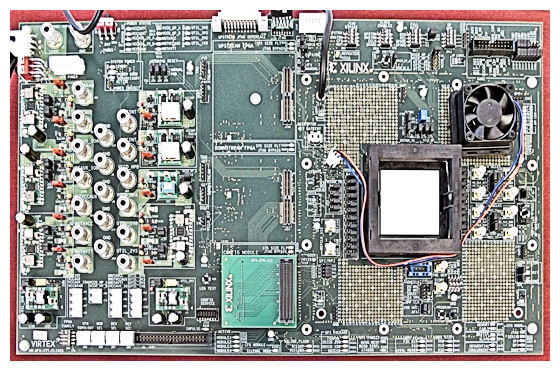
\includegraphics[height=60mm]{Figures/fpga.jpg}

% Title, author and degree
\vspace{0.8cm}
{\FontLb C Compiler for the VERSAT Reconfigurable Processor} \\
\vspace{3.6cm}
{\FontMb Gonçalo da Conceição Reis dos Santos} \\
\vspace{1.9cm}
{\FontLn Thesis to obtain the Master of Science Degree in} \\
\vspace{0.3cm}
{\FontLb Electrical and Computer Engineering} \\
%\vspace{1.9cm}
\vspace{1.0cm}
{\FontSn %
\begin{tabular}{ll}
Supervisor: & Prof. José João Henriques Teixeira de Sousa
\end{tabular} } \\
\vspace{1.0cm}
{\FontMb Examination Committee} \\
\vspace{0.3cm}
{\FontSn %
\begin{tabular}{ll}
Chairperson: & Prof. Francisco André Corrêa Alegria\\
Supervisor: & Prof. José João Henriques Teixeira de Sousa \\
Member of the Committee: & Prof. Paulo Ferreira Godinho Flores \\
\end{tabular} } \\
\vspace{1.5cm}
{\FontMb November 2019} \\
%
\end{center}

\cleardoublepage
 % file "Thesis_FrontCover.tex"
\cleardoublepage

% ----------------------------------------------------------------------
% Dedication page (optional)
% ----------------------------------------------------------------------
%%%%%%%%%%%%%%%%%%%%%%%%%%%%%%%%%%%%%%%%%%%%%%%%%%%%%%%%%%%%%%%%%%%%%%%%%
%                                                                      %
%     File: Thesis_Dedication.tex                                      %
%     Tex Master: Thesis.tex                                           %
%                                                                      %
%     Author: Andre C. Marta                                           %
%     Last modified :  2 Jul 2015                                      %
%                                                                      %
%%%%%%%%%%%%%%%%%%%%%%%%%%%%%%%%%%%%%%%%%%%%%%%%%%%%%%%%%%%%%%%%%%%%%%%%

\null\vskip5cm%
\begin{flushright}
     Dedicated to someone special...
\end{flushright}
\vfill\newpage

 % file "Thesis_Dedication.tex"
%\cleardoublepage

% ----------------------------------------------------------------------
%  Acknowledgments (optional)
% ----------------------------------------------------------------------
%%%%%%%%%%%%%%%%%%%%%%%%%%%%%%%%%%%%%%%%%%%%%%%%%%%%%%%%%%%%%%%%%%%%%%%%%
%                                                                      %
%     File: Thesis_Acknowledgments.tex                                 %
%     Tex Master: Thesis.tex                                           %
%                                                                      %
%     Author: Andre C. Marta                                           %
%     Last modified :  2 Jul 2015                                      %
%                                                                      %
%%%%%%%%%%%%%%%%%%%%%%%%%%%%%%%%%%%%%%%%%%%%%%%%%%%%%%%%%%%%%%%%%%%%%%%%

\section*{\acknowledgments}

% Add entry in the table of contents as section
\addcontentsline{toc}{section}{\acknowledgments}

I want to thank my supervisor, Professor José Teixeira de Sousa, for the 
opportunity to develop this work and for his guidance and support during that process. 
His help was fundamental to overcome the multiple obstacles that I faced during this work.

I also want to acknowledge Professor Horácio Neto for providing a simple Convolutional 
Neural Network application, used as a basis for the application developed for the 
RV32-Versat architecture.

A special acknowledgement goes to my friends, for their continuous support, and Válter,  
that is developing a multi-layer architecture for RV32-Versat. When everything seemed to 
be doomed he always had a miraculous solution.

Finally, I want to express my sincere gratitude to my family for giving me all the 
support and encouragement that I needed throughout my years of study and through the 
process of researching and writing this thesis. They are also part of this work.\\

\textbf{Thank you.}

 % file "Thesis_Acknowledgements.tex"
%\cleardoublepage

% ----------------------------------------------------------------------
%  Abstract (both in English and Portuguese)
% ----------------------------------------------------------------------
%%%%%%%%%%%%%%%%%%%%%%%%%%%%%%%%%%%%%%%%%%%%%%%%%%%%%%%%%%%%%%%%%%%%%%%%%
%                                                                      %
%     File: Thesis_Resumo.tex                                          %
%     Tex Master: Thesis.tex                                           %
%                                                                      %
%     Author: Carlos A. Rodrigues                                           %
%     Last modified : 21 Jan 2011                                      %
%                                                                      %
%%%%%%%%%%%%%%%%%%%%%%%%%%%%%%%%%%%%%%%%%%%%%%%%%%%%%%%%%%%%%%%%%%%%%%%%

\section*{Resumo}

% Add entry in the table of contents as section
\addcontentsline{toc}{section}{Resumo}

Inserir o resumo em Portugu\^{e}s aqui com o máximo de 250 palavras e acompanhado de 4 a 6 palavras-chave...

\vfill

\textbf{\Large Palavras-chave:} OpenRISC, Sistema em um chip,...

\cleardoublepage

   % file "Thesis_Resumo.tex"
%\cleardoublepage

%%%%%%%%%%%%%%%%%%%%%%%%%%%%%%%%%%%%%%%%%%%%%%%%%%%%%%%%%%%%%%%%%%%%%%%%
%                                                                      %
%     File: Thesis_Abstract.tex                                        %
%     Tex Master: Thesis.tex                                           %
%                                                                      %
%     Author: Andre C. Marta                                           %
%     Last modified :  2 Jul 2015                                      %
%                                                                      %
%%%%%%%%%%%%%%%%%%%%%%%%%%%%%%%%%%%%%%%%%%%%%%%%%%%%%%%%%%%%%%%%%%%%%%%%

\section*{Abstract}

% Add entry in the table of contents as section
\addcontentsline{toc}{section}{Abstract}

Versat is a Coarse-Grain Reconfigurable Array architecture (CGRA), which
implements self and partial reconfiguration by using a simple controller
unit. This report studies the current state of the art in HDL and CGRA
simulation, providing a basis to the development of a simulation environment for
Versat. The main objective of this environment is to provide a faster way to
develop and debug software without the use of prototyping hardware. Therefore,
the two types of HDL simulators, event-driven and cycle-accurate, their
advantages and disadvantages are studied, along with a performance comparison
between them. A study of high-level implementations for CGRA simulation is
also presented.

\vfill

\textbf{\Large Keywords:} Versat, coarse-grain reconfigurable arrays, HDL
simulation, CGRA simulation, high-level simulation

 % file "Thesis_Abstract.tex"
\cleardoublepage

% ----------------------------------------------------------------------
%  Table of contents, list of tables, list of figures and nomenclature
% ----------------------------------------------------------------------

% Table of contents
%
\tableofcontents
\cleardoublepage 

% List of tables
%
% Add entry in the table of contents as section
\phantomsection
\addcontentsline{toc}{section}{\listtablename}
% Generate list
\listoftables
\cleardoublepage 

% List of figures
%
% Add entry in the table of contents as section
\phantomsection
\addcontentsline{toc}{section}{\listfigurename}
% Generate list
\listoffigures
\cleardoublepage 

% Nomenclature
%
% entries of nomenclature list
%%%%%%%%%%%%%%%%%%%%%%%%%%%%%%%%%%%%%%%%%%%%%%%%%%%%%%%%%%%%%%%%%%%%%%%%%
%                                                                      %
%     File: Thesis_Nomenclature.tex                                    %
%     Tex Master: Thesis.tex                                           %
%                                                                      %
%     Author: Gonçalo Santos                                           %
%     Last modified : 20 Oct 2018                                      %
%                                                                      %
%%%%%%%%%%%%%%%%%%%%%%%%%%%%%%%%%%%%%%%%%%%%%%%%%%%%%%%%%%%%%%%%%%%%%%%%
%
% The definitions can be placed anywhere in the document body
% and their order is sorted by <symbol> automatically when
% calling makeindex in the makefile
%
% The \glossary command has the following syntax:
%
% \glossary{entry}
%
% The \nomenclature command has the following syntax:
%
% \nomenclature[<prefix>]{<symbol>}{<description>}
%
% where <prefix> is used for fine tuning the sort order,
% <symbol> is the symbol to be described, and <description> is
% the actual description.

% ----------------------------------------------------------------------
% Roman symbols [r]
\nomenclature[ru]{$\bf u$}{Velocity vector.}
\nomenclature[ru]{$u,v,w$}{Velocity Cartesian components.}
\nomenclature[rp]{$p$}{Pressure.}
\nomenclature[rC]{$C_D$}{Coefficient of drag.}
\nomenclature[rC]{$C_L$}{Coefficient of lift.}
\nomenclature[rC]{$C_M$}{Coefficient of moment.}

% ----------------------------------------------------------------------
% Greek symbols [g]
\nomenclature[g]{$\rho$}{Density.}
\nomenclature[g]{$\alpha$}{Angle of attack.}
\nomenclature[g]{$\beta$}{Angle of side-slip.}
\nomenclature[g]{$\mu$}{Molecular viscosity coefficient.}
\nomenclature[g]{$\kappa$}{Thermal conductivity coefficient.}

% ----------------------------------------------------------------------
% Subscripts [s]
\nomenclature[s]{$x,y,z$}{Cartesian components.}
\nomenclature[s]{$i,j,k$}{Computational indexes.}
\nomenclature[s]{$\infty$}{Free-stream condition.}
\nomenclature[s]{ref}{Reference condition.}
\nomenclature[s]{$n$}{Normal component.}

% ----------------------------------------------------------------------
% Supercripts [t]
\nomenclature[t]{T}{Transpose.}
\nomenclature[t]{*}{Adjoint.}

 % file "Thesis_Nomenclature.tex"
%
% Add entry in the table of contents as section
%\phantomsection
%\addcontentsline{toc}{section}{\nomname}
% Insert glossary/nomenclature section produced by MakeIndex
%\printnomenclature
%\cleardoublepage

% entries of glossary list
%%%%%%%%%%%%%%%%%%%%%%%%%%%%%%%%%%%%%%%%%%%%%%%%%%%%%%%%%%%%%%%%%%%%%%%%%
%                                                                      %
%     File: Thesis_Glossary.tex                                        %
%     Tex Master: Thesis.tex                                           %
%                                                                      %
%     Author: Carlos A. Rodrigues                                           %
%     Last modified : 30 Oct 2012                                      %
%                                                                      %
%%%%%%%%%%%%%%%%%%%%%%%%%%%%%%%%%%%%%%%%%%%%%%%%%%%%%%%%%%%%%%%%%%%%%%%%
%
% The definitions can be placed anywhere in the document body
% and their order is sorted by <symbol> automatically when
% calling makeindex in the makefile
%
% The \glossary command has the following syntax:
%
% \glossary{entry}
%
% The \nomenclature command has the following syntax:
%
% \nomenclature[<prefix>]{<symbol>}{<description>}
%
% where <prefix> is used for fine tuning the sort order,
% <symbol> is the symbol to be described, and <description> is
% the actual description.

% ----------------------------------------------------------------------

\glossary{name={\textbf{MDO}},description={Multi-Disciplinar Optimization is an engineering technique that uses optimization methods to solve design problems incorporating two or more disciplines.}}

\glossary{name={\textbf{CFD}},description={Computational Fluid Dynamics is a branch of fluid mechanics that uses numerical methods and algorithms to solve problems that involve fluid flows.}}

\glossary{name={\textbf{CSM}},description={Computational Structural Mechanics is a branch of structure mechanics that uses numerical methods and algorithms to perform the analysis of structures and its components.}}

 % file "Thesis_Glossary.tex"

% Add entry in the table of contents as section
%\phantomsection
%\addcontentsline{toc}{section}{\glossaryname}
% Insert glossary section produced by MakeIndex
%\printglossary
%\cleardoublepage

% Set arabic numbering (1,2,...) after preface
%
\setcounter{page}{1}
\pagenumbering{arabic}

% ----------------------------------------------------------------------
%  Chapters
% ----------------------------------------------------------------------

%%%%%%%%%%%%%%%%%%%%%%%%%%%%%%%%%%%%%%%%%%%%%%%%%%%%%%%%%%%%%%%%%%%%%%%%
%                                                                      %
%     File: Thesis_Introduction.tex                                    %
%     Tex Master: Thesis.tex                                           %
%                                                                      %
%     Author: Andre C. Marta                                           %
%     Last modified :  2 Jul 2015                                      %
%                                                                      %
%%%%%%%%%%%%%%%%%%%%%%%%%%%%%%%%%%%%%%%%%%%%%%%%%%%%%%%%%%%%%%%%%%%%%%%%

\chapter{Introduction}
\label{chapter:introduction}




In this report, the problem of accelerating the execution of Deep Neural
Networks (DNNs) using Coarse GRained Reconfigurable Arrays (CGRAs) is studied,
with special emphasis on compiling a DNN description into code that runs on
CPU/CGRA system. The Deep Versat Architecture~\cite{valter:deepversat} CGRA will be used as an
implementation tool in this work.


%%%%%%%%%%%%%%%%%%%%%%%%%%%%%%%%%%%%%%%%%%%%%%%%%%%%%%%%%%%%%%%%%%%%%%%%
\section{Problem}
\label{section:problem}

Neural Networks have been an object of study since the 1940's, but until the
beginning of this decade their applications were limited and did not play a
major role in computer vision conferences. With its meteoric rise in research,
several solutions to accelerate this algorithm have appeared, from Field Programmable Gate Arrays (FPGA) to
Application Specific Integrated Circuits (ASIC) implementations.

Convolutional Neural Networks (CNNs) are a particular kind of DNN where the output
values of the neurons in one layer are convolved with a kernel to produce the
input values of the neurons of the next layer. This algorithm is compute bound,
that is, its performance depends on how fast it can do certain calculations, and
depend less on the memory access time. Namely the convolutional layers take
approximately 90$\%$ of the computation time.

The acceleration of these workloads is a matter of importance for today's
applications such as image processing for object recognition or simply to
enhance certain images. Other uses like instant translation and virtual
assistants are applications of neural networks and their acceleration is of
vital importance to bring them into Internet of Things.

A suitable circuit to accelerate DNNs in hardware is the CGRA. A CGRA is a
collection of Functional Units and memories with programmable interconnections
in order to form computational datapaths. A CGRA can be implemented in both
FPGAs and ASICs. CGRAs can be reconfigured much faster than FPGAs, as they have
much less configuration bits. If reconfiguration is done at runtime, CGRAs add
temporal scalability to the spacial scalability that characterize
FPGAs. Moreover, partial reconfiguration is much easier to do in CGRAs compared
to FPGAs which further speeds up reconfiguration time. Another advantage of
CGRAs is the fact that they can be programmed entirely in software, contrasting
with the large development time of customized Intellectual Property (IP) blocks.
The Coarse Grain Reconfigurable Arrays (CGRA) is a midway acceleration solution
between FPGAs, which are flexible but large, power hungry and difficult to
reprogram, and ASICs, which are fast but generally not programmable.

However, mapping a specific DNN to a CGRA requires knowledge of its
architecture, latencies and register configurations, which may become a lengthy
process, especially if the user wants to explore the design space for several
DNN configurations. An automatic compiler that can map a standard DNN
description into CPU/CGRA code would dramatically decrease time to market of its
users. Currently there are equivalent tools for CPUs and GPUs and
even for FPGAS.


%%%%%%%%%%%%%%%%%%%%%%%%%%%%%%%%%%%%%%%%%%%%%%%%%%%%%%%%%%%%%%%%%%%%%%%%
\section{Solution}
\label{section:solution}

The proposed solution is a compiler that takes a configuration file from a
neural network framework like Caffe or Darknet. This new tool inputs the
parameters of Deep Versat, such as the number of layers and functional units,
and produces the C code needed for the Versat runs. This code is run on the
RISC-V picorv32~\cite{picorv} CPU controller that has Deep Versat as a peripheral.

%%%%%%%%%%%%%%%%%%%%%%%%%%%%%%%%%%%%%%%%%%%%%%%%%%%%%%%%%%%%%%%%%%%%%%%%
%\section{Thesis Outline}
%\label{section:outline}

%Briefly explain the contents of the different chapters...

%%%%%%%%%%%%%%%%%%%%%%%%%%%%%%%%%%%%%%%%%%%%%%%%%
%\section{Author's Work}
%\label{section:authorwork}

%TO ADD----

%%%%%%%%%%%%%%%%%%%%%%%%%%%%%%%%%%%%%%%%%%%%%%%%%%
\section{Report Outline}
\label{reportoutline}

This report is composed of 4 more chapters. In the second chapter, the
state-of-the-art of neural networks and the difficulties accelerating them is
described. In the third chapter, the Deep Versat architecture and how to program
it is explained. In the fourth chapter, CNN compiler techniques are
explored. Finally, the last chapter contains the proposed solution and the plan
for its execution.


 % file "Thesis_Introduction.tex"
\cleardoublepage

%%%%%%%%%%%%%%%%%%%%%%%%%%%%%%%%%%%%%%%%%%%%%%%%%%%%%%%%%%%%%%%%%%%%%%%%
%                                                                      %
%     File: Thesis_Versat.tex                                      %
%     Tex Master: Thesis.tex                                           %
%                                                                      %
%     Author: Andre C. Marta                                           %
%     Last modified :  2 Jul 2015                                      %
%                                                                      %
%%%%%%%%%%%%%%%%%%%%%%%%%%%%%%%%%%%%%%%%%%%%%%%%%%%%%%%%%%%%%%%%%%%%%%%%

\chapter{The Versat architecture}
\label{chapter:versat}

\begin{figure}[!htb]
	\centering
	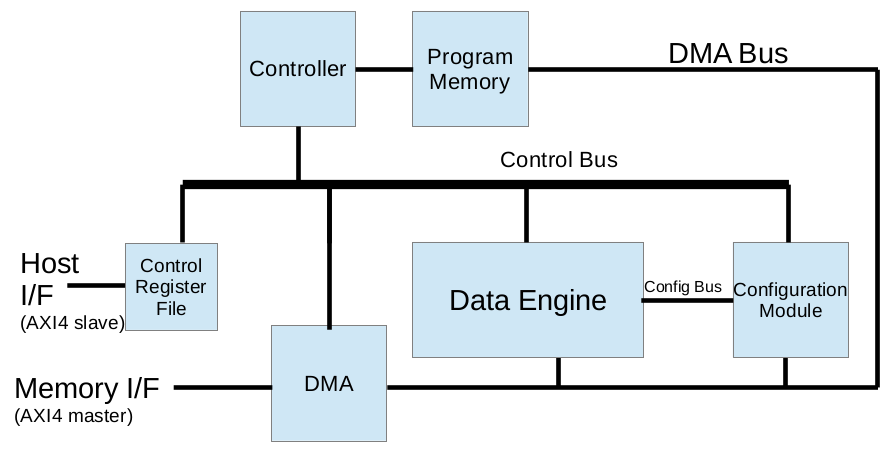
\includegraphics[width=0.8\textwidth]{Figures/top.png}
	\caption{Versat top-level entity.}
	\label{fig:top}
\end{figure}

The Versat architecture~\cite{sousa:versat, sousa:versat2016, sousa:controller,
  sousa:compiler} is shown in Figure~\ref{fig:top}, and it consists of the
following modules: Controller, Program Memory, Control Register File, DMA, Data
Engine and Configuration Module. The Controller can access the various modules
in the system via the Control Bus, and it executes programs stored in the
Program Memory (9kB = 1kB boot ROM + 8kB RAM). The user programs are loaded in
the RAM to execute algorithms which involve managing Data Engine (DE)
reconfigurations and DMA data transfers.

Versat user programs can use the DE to carry out data intensive computations. To
perform these computations, the Controller writes DE configurations to the
Configuration Module (CM) or simply restores configurations previously stored in
the CM. The Controller can also load the DE with data to be processed or save
the processed data back in the external memory using the DMA engine. The DMA
engine can also be used to initially load the Versat program or to move CGRA
configurations between the core and the external memory.

The Versat core has a host and a memory interface. Both of them use ARM’s
Advanced eXtensible Interface (AXI), a standard for busing. The host interface
(AXI slave) is used by a host system to instruct Versat to load and execute
programs. The host and the Controller communicate using the Control Register
File (CRF), an unit that is also used by Versat programs as a general purpose
(1-cycle access) register file. The memory interface (AXI master) is used to
access data from an external memory using the DMA.



%%%%%%%%%%%%%%%%%%%%%%%%%%%%%%%%%%%%%%%%%%%%%%%%%%%%%%%%%%%%%%%%%%%%%%%%
\section{Data Engine}
\label{section:data}

\begin{figure}[!htb]
	\centering
	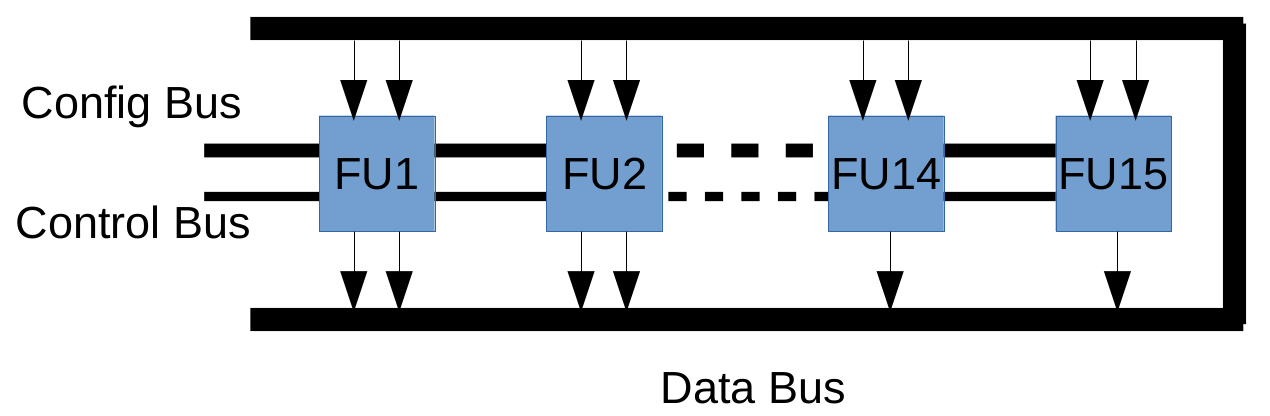
\includegraphics[width=0.8\textwidth]{Figures/de.png}
	\caption{Versat data engine.}
	\label{fig:de}
\end{figure}

The Data Engine (DE) has a flexible topology, in which the user can configure
the amount of functional units (FUs) and their respective type. In
Figure~\ref{fig:de} is shown a DE example with 15 FUs. The DE is a 32-bit
architecture with the following configurable FUs: Arithmetic and Logic Unit
(ALU), Multiplier Accumulator (MAC), Barrel Shifter (BS) and dual-port 16kB
embedded memories (MEM). The output registers of the FUs are read/write
accessible by the Controller via the Control Bus.

The FUs are interconnected by a wide bus called the Data Bus. This bus is the
concatenation of all FU outputs, with each FU contributing with a 32-bit section
to the Data Bus. An embedded memory contributes 2 sections to the Data Bus,
since it has 2 ports. These sections can be selected by each FU, according to
the configurations that they receive from the respective configuration registers
in the CM, whose outputs are concatenated in another wide bus called the Config
Bus.

The DE has a full mesh topology, meaning that each FU can select any FU output
as one of its inputs. This kind of structure may seem unnecessary but it greatly
simplifies the compiler design as it avoids expensive place and route
algorithms~\cite{sousa:versat2016}.

\begin{figure}[!htb]
	\centering
	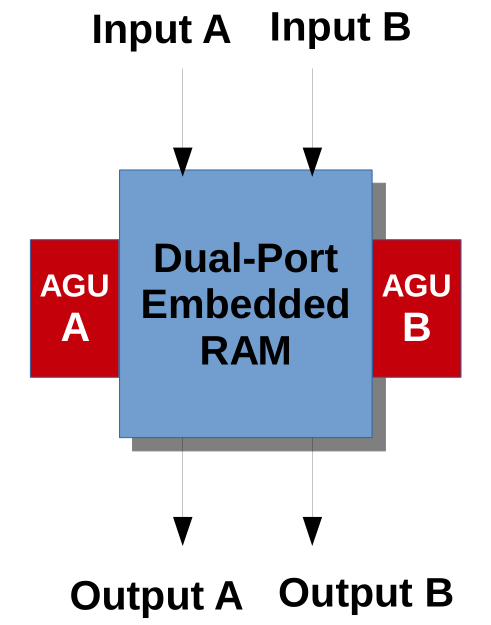
\includegraphics[width=0.23\textwidth]{Figures/memory.png}
	\caption{Versat dual-port embedded memory with AGUs.}
	\label{fig:memory}
\end{figure}

Each one of the dual-port memories used in Versat have a data input, a data
output and an address input, as shown in Figure~\ref{fig:memory}. Also, each
port has an Address Generation Unit (AGU), that can be programmed to generate
the address sequence used to access data from the memory port during the
execution of a program loop in the DE. The AGUs support two levels of nested
loops and can start execution with a programmable delay, so that circuit paths
with different latencies can be synchronized.

%%%%%%%%%%%%%%%%%%%%%%%%%%%%%%%%%%%%%%%%%%%%%%%%%%%%%%%%%%%%%%%%%%%%%%%%
\section{Configuration Module}
\label{section:configuration}

\begin{figure}[!htb]
	\centering
	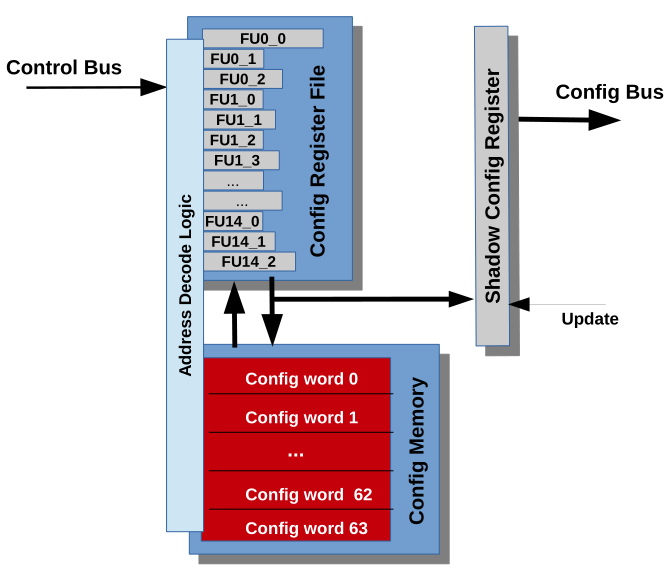
\includegraphics[width=0.6\textwidth]{Figures/configuration.png}
	\caption{Versat configuration module example.}
	\label{fig:cm}
\end{figure}

In Versat, the configuration bits are organized in configuration spaces, one for
each FU. Each configuration space comprises multiple fields, which are memory
mapped from the Controller point of view. Thus, the Controller is able to change
a single configuration field of an FU by writing to the respective address. This
implements partial reconfiguration.

A Configuration Module (CM) example is illustrated in Figure~\ref{fig:cm}, with
a reduced number of configuration spaces and fields for simplicity. It contains
a register file with a variable length (the length depends on the FUs used), a
shadow register and a memory. The shadow register holds the current
configuration of the DE, which is copied from the main configuration register
whenever the Update signal is activated. This means that the configuration
register can be changed in the main register while the DE is running.

When the CM is addressed by the Controller, the decode logic checks if the
configuration register file or the configuration memory is being addressed. The
configuration register file accepts write requests and ignores read requests. On
the other hand, the configuration memory deals with read and write requests in
the following way: a read request causes the addressed contents of the
configuration memory to be transferred into the configuration register file,
while a write request causes the contents of the configuration register file to
be stored into the addressed position of the configuration memory. This is a
mechanism for saving and loading entire configurations in a single clock cycle
because all the data transfers are internal.

%%%%%%%%%%%%%%%%%%%%%%%%%%%%%%%%%%%%%%%%%%%%%%%%%%%%%%%%%%%%%%%%%%%%%%%%
\section{Controller}
\label{section:controller}

\begin{figure}[!htb]
	\centering
	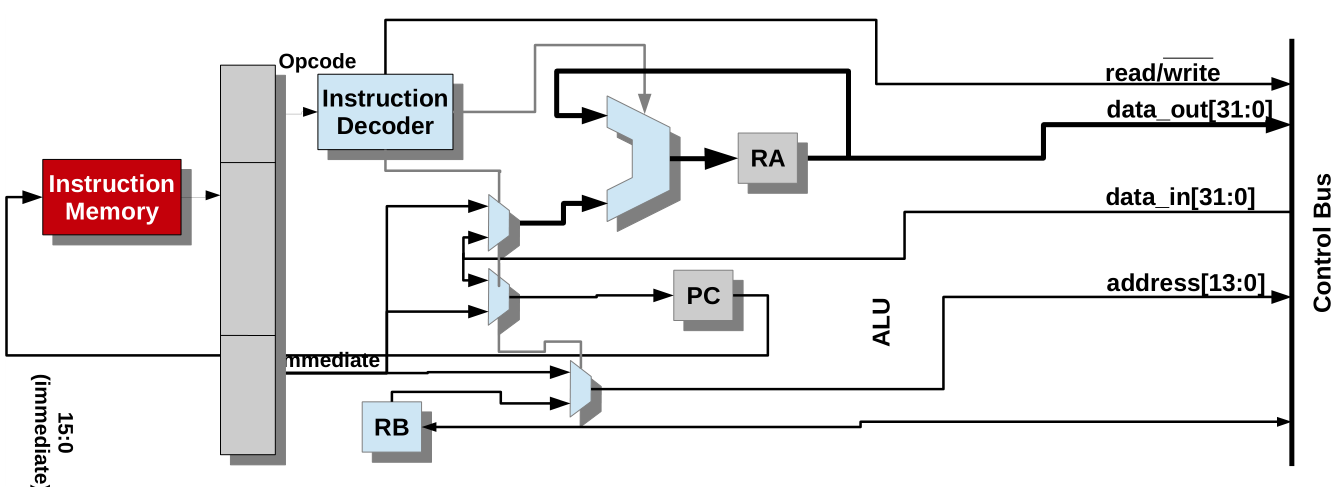
\includegraphics[width=0.8\textwidth]{Figures/controller.png}
	\caption{Versat controller.}
	\label{fig:controller}
\end{figure}

The controller used in the Versat architecture is just used for reconfiguration,
data transfer and simple algorithmic control. This controller is not meant to
replace a more general host processor, which can run complex applications while
using Versat as an accelerator.

The controller has an accumulator architecture, using a 2 stage pipeline, as
shown in Figure~\ref{fig:controller}. In this architecture 3 main registers are
used: RA, RB and PC. The RA is the accumulator, the RB is the address register,
used for indirect loads and stores, and the PC is the register that holds the
value of the program counter.

The controller is the master of a simple bus called the Control Bus, which can
be accessed using the 4 signals shown in Figure~\ref{fig:controller}. Register
RB can be accessed using the Control Bus as if it were a peripheral of the
Control Bus.

\begin{table}[!htbp]
	\centering
	\caption{Versat instruction set.}
	\label{tab:isa}
	\begin{tabular}{|c|l|}
		\hline 
		{\bf Mnemonic} & {\bf Description} \\
		\hline \hline 
		rdw & RA = (Imm)\\
		\hline
		wrw & (Imm) = RA\\
		\hline
		rdwb & RA = (RB)\\
		\hline
		wrwb & (RB) = RA\\
		\hline
		ldi & RA = Imm\\
		\hline
		ldih & RA[31:16] = Imm\\
		\hline
		beqi & RA == 0? PC = Imm: PC += 1; RA = RA-1\\
		\hline
		beq & RA == 0? PC = (Imm): PC += 1; RA = RA-1\\
		\hline
		bneqi & RA != 0? PC = Imm: PC += 1; RA = RA-1\\
		\hline
		bneq & RA != 0? PC = (Imm): PC += 1; RA = RA-1\\
		\hline
		add & RA = RA + (Imm)\\
		\hline
		addi & RA = RA + Imm\\
		\hline
		sub & RA = RA - (Imm)\\
		\hline
		shft & RA = (Imm $<$ 0)? RA=RA$<<$1: RA=RA$>>$1\\
		\hline
		and & RA = RA \& (Imm)\\
		\hline
		xor & RA = RA \^ (Imm)\\
		\hline
	\end{tabular}
\end{table}

The Versat controller Instruction Set Architecture (ISA) has 16 instructions, as
shown in Table~\ref{tab:isa}. Currently, it can only be programmed in assembly
language as it does not yet have a C compiler which is being developed by
another student working in this project.


%%%%%%%%%%%%%%%%%%%%%%%%%%%%%%%%%%%%%%%%%%%%%%%%%%%%%%%%%%%%%%%%%%%%%%%%
\section{Application Example}
\label{section:application}

During the work carried out for this report an application for an international
client using the Versat architecture was developed. It consists of an MP3
encoder, shown in Figure~\ref{fig:application}, where Versat is used to
accelerate the front end of the algorithm, denoted MP3-FE in
Figure~\ref{fig:application}).

\begin{figure}[!htb]
	\centering
	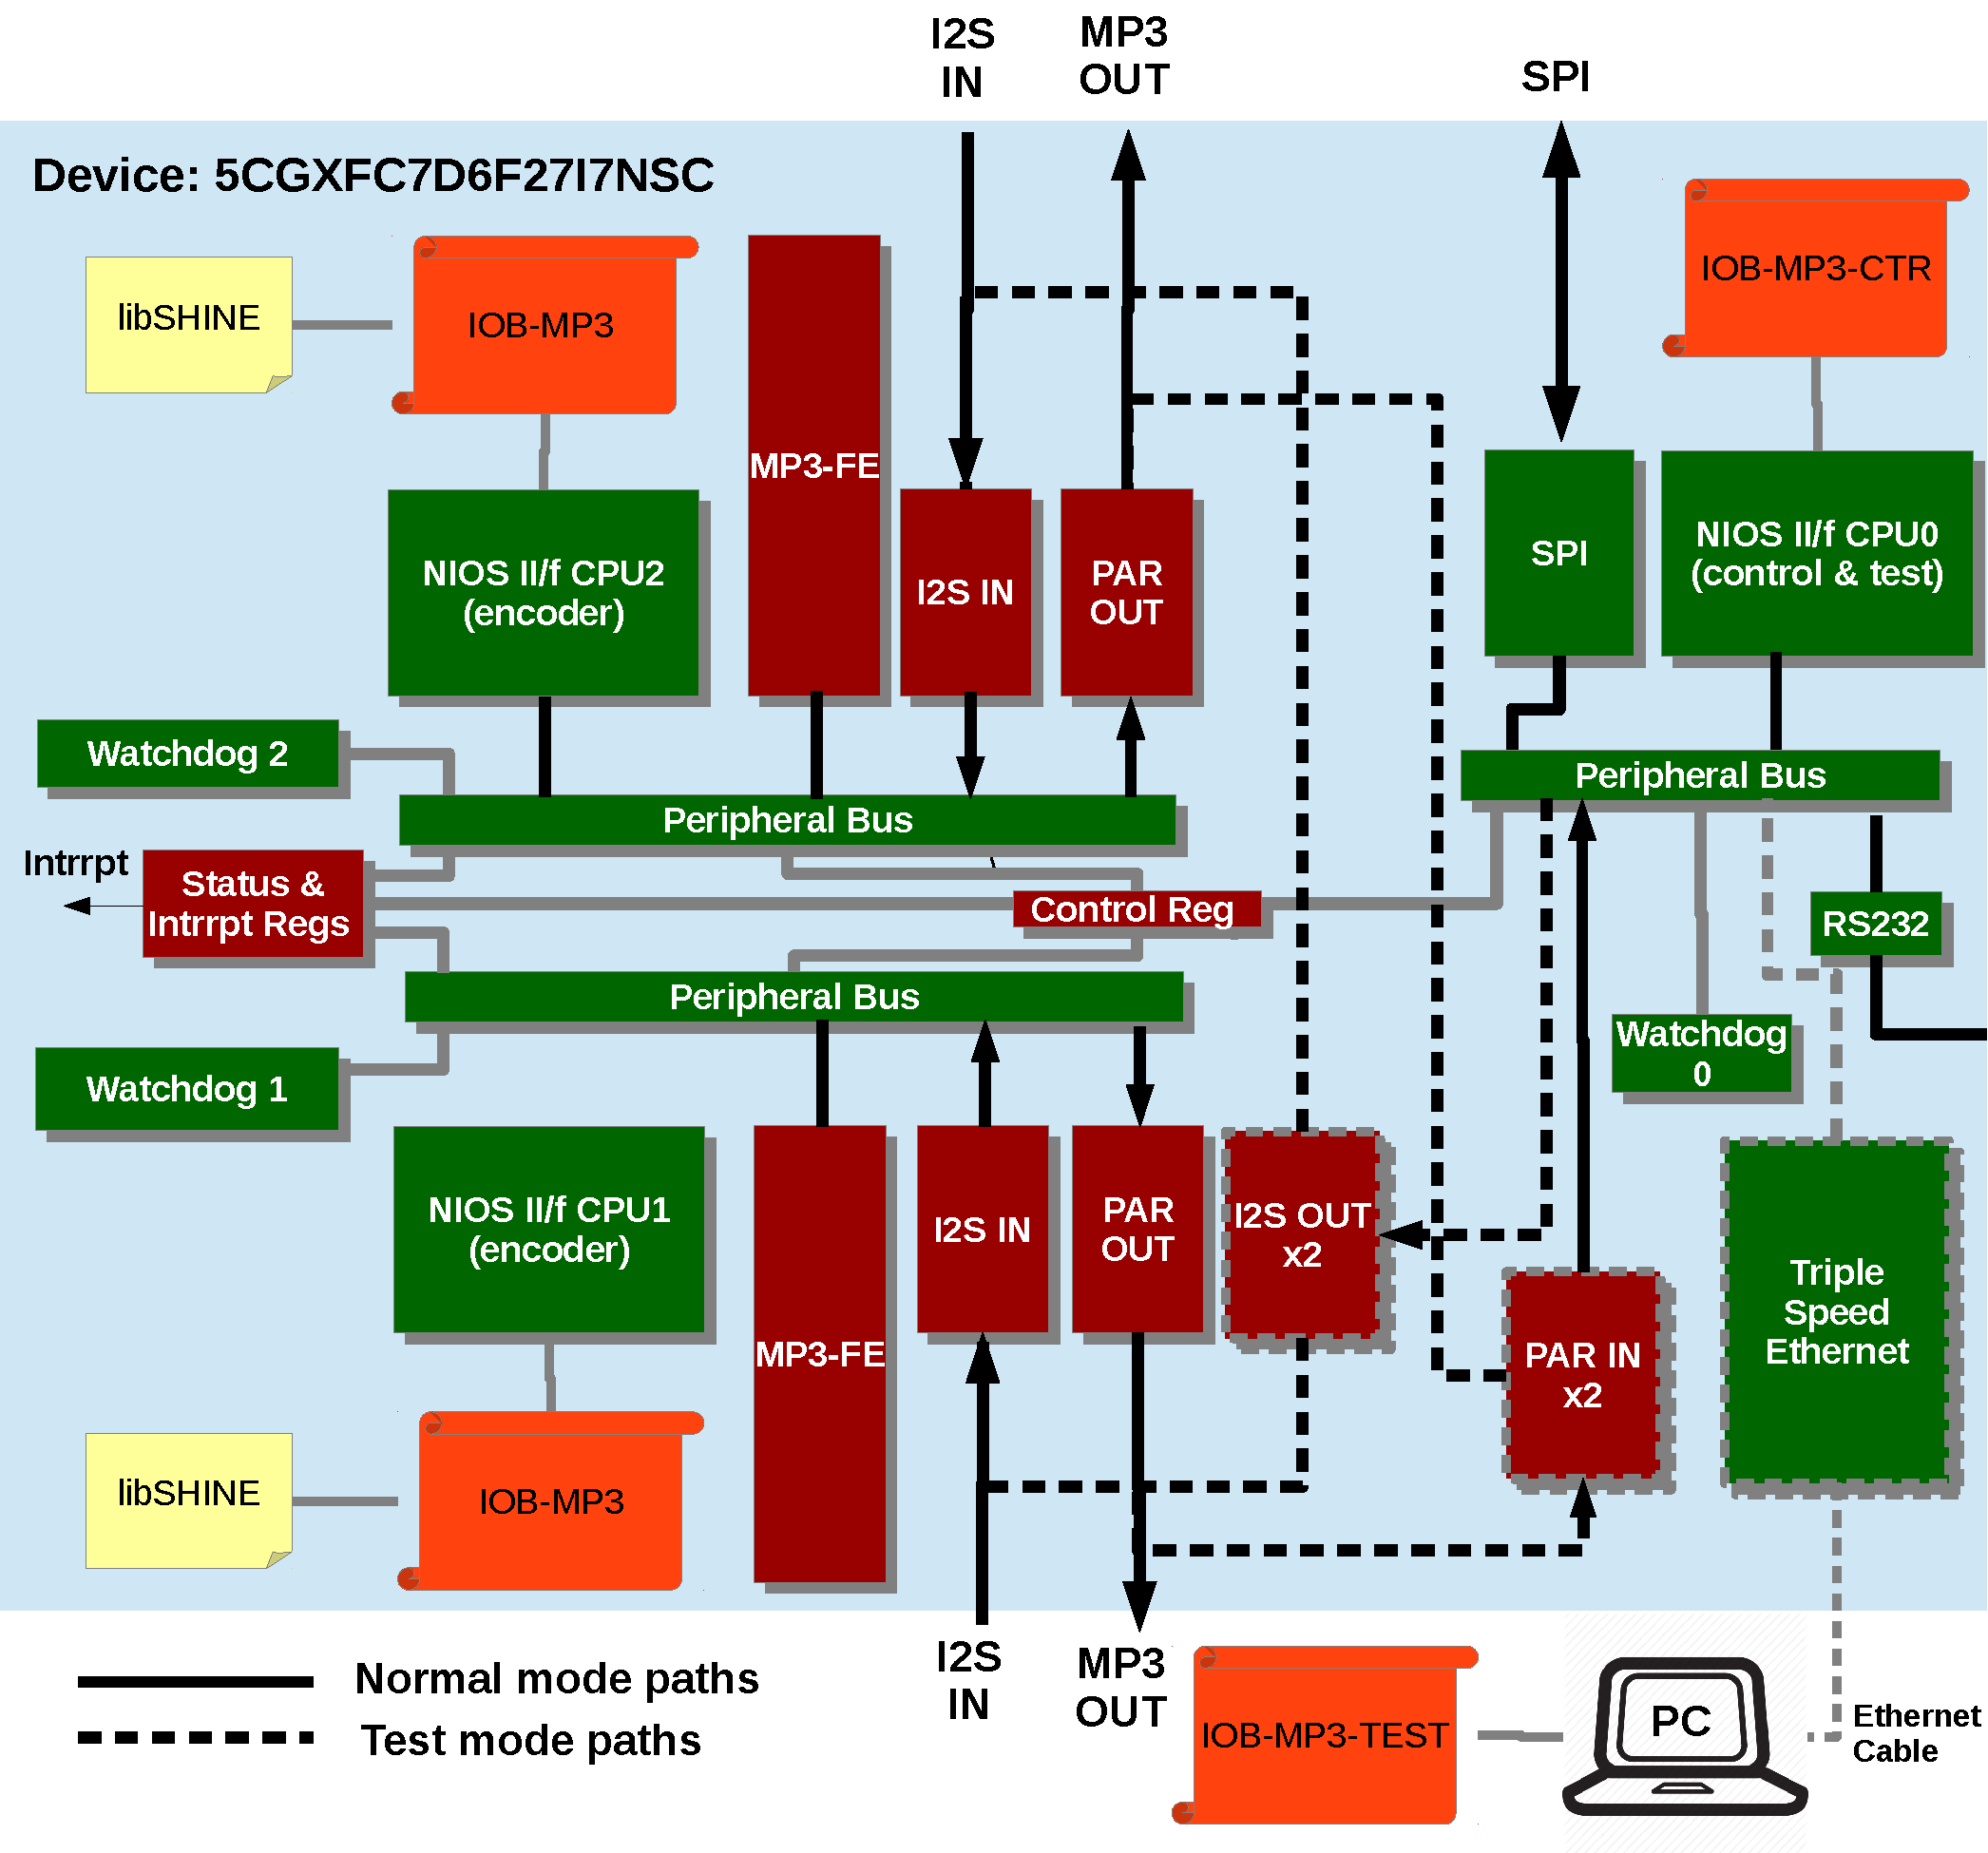
\includegraphics[width=0.85\textwidth]{Figures/bd.pdf}
	\caption{Schematic of the application where Versat was used.}
	\label{fig:application}
\end{figure}

The MP3 algorithm is based in Shine~\cite{shine:mp3}, a fast fixed-point MP3
encoding library. The front end runs sub-band filtering of the audio signal and
applies the Modified Discrete Cosine Transform to the result. These functions
are the most computationally expensive functions in the MP3 algorithm and
normally require DSP extensions to the ISA of the processor used. In the
approach taken, a more modest processor was used (Intel's NIOS2) which used
Versat as a peripheral acceleration core.

To run this algorithm the Versat architecture was configured with 4 dual-port
memories and 3 FUs: a Multiply Accumulate Unit (MAC), a simple Arithmetic and
Logic Unit (ALU) and a Barrel Shifter Unit (BS). The MP3 front-end was written
in the Versat Assembly language, since Versat compiler does not support yet the
use of a higher level programming language (like C or C++).

The FE was intensively simulated before synthesis and implementation in the
FPGA. Initially, the simulations were performed using Icarus
Verilog~\cite{icarus:verilog}, an open-source Verilog simulator. However, as the
complexity of the core increased, the simulation times also increased
dramatically, since Icarus Verilog is a fairly slow simulator, as will be seen
in section~\ref{section:performance}, where the performance of the different HDL
simulators is analysed.

As a result, at a certain point in the project, the simulator was changed to
Cadence NCSim~\cite{cadence:ncsim} to speed up the simulations. Despite NCsim
being considerably faster than Icarus Verilog, the simulations still took a
considerable amount of time. This reinforces the need for a faster simulation
environment for the Versat architecture.
 % file "Thesis_Versat.tex"
\cleardoublepage

%%%%%%%%%%%%%%%%%%%%%%%%%%%%%%%%%%%%%%%%%%%%%%%%%%%%%%%%%%%%%%%%%%%%%%%%
%                                                                      %
%     File: Thesis_Versat.tex                                          %
%     Tex Master: Thesis.tex                                           %
%                                                                      %
%     Author: Andre C. Marta                                           %
%     Last modified :  2 Jul 2015                                      %
%                                                                      %
%%%%%%%%%%%%%%%%%%%%%%%%%%%%%%%%%%%%%%%%%%%%%%%%%%%%%%%%%%%%%%%%%%%%%%%%

\chapter{HDL Simulators}
\label{chapter:simulators}

As mentioned before, HDL simulators play a fundamental role during the different
phases of circuit development, and there are multiple simulation tools that can
be used. However, despite all these tools having more or less the same purpose
(provide a way to validate the circuit being tested), they do not work in the
same way.

Typically, before testing a circuit, a test bench is created. The test bench is
a program, written in a HDL or in a programming language (like SystemC, for
example), that comprises three modules~\cite{tan:vhstas}: stimuli generator,
golden response generator and response analyser, as shown in
Figure~\ref{fig:tb}. The stimuli generator module is responsible for generating
the signals needed to make the circuit work properly. On the other hand, the
golden response generator computes the expected circuit response, based on the
inputs generated by the stimuli generator. Finally, the response analyzer
compares the circuit output signals with the ones generated by the golden
response generator. During simulation, if both signs are equal, it means that
the circuit is working as intended.

\begin{figure}[!htb]
	\centering
	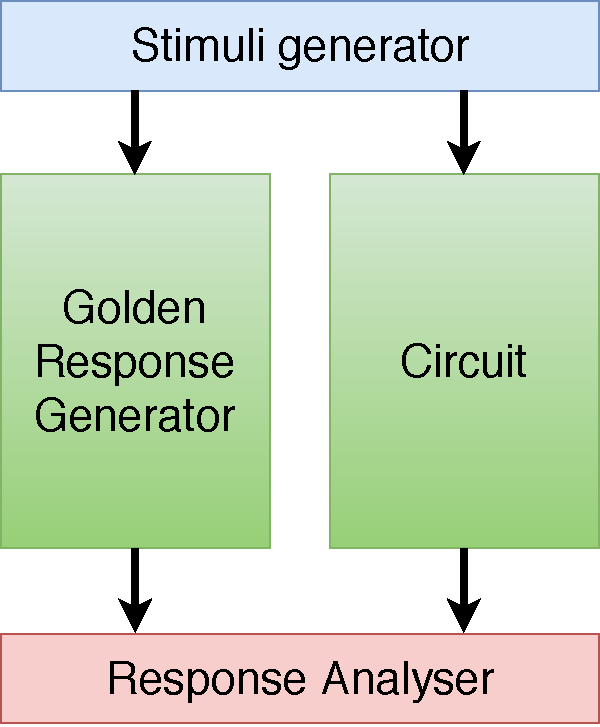
\includegraphics[width=0.42\textwidth]{Figures/Testbench.pdf}
	\caption{Test bench diagram.}
	\label{fig:tb}
\end{figure}

The results provided by the test-bench might depend on the chosen
simulator. This happens because all the simulators work in different ways: while
some focus on obtaining the most complete results (including simulation
timings), sacrificing the speed of the simulations, others do the opposite. In
this perspective, the simulators can be divided into two main categories~\cite{tan:vhstas,palnitkar:verilog}: event-driven or cycle-accurate.

\section{Event-Driven Simulators}
\label{section:event}

The first category of simulators are the event-driven
ones~\cite{tan:vhstas,gunes:survey,palnitkar:verilog}. This simulators work by
taking events sequentially, propagating them through the circuit until it
reaches a steady state.

The events are generated each time that a circuit input is changed, being stored
in a queue, ordered chronologically to allow the correct execution of the
events. When an event is evaluated, only the circuit nodes that have their input
changed by that event are evaluated. After evaluation, the event is removed from
the queue, with new events resultant from the output changes being added. This
means that the same element might be evaluated multiple times during the same
time step due to the feedback from some signals.

It's important to mention that during the simulation process there's a timer
that is used to keep track of the events timings. This leads to one of the main
advantages of event-driven simulation, which is the accurate simulation results,
with detailed timing information, allowing the identification of timing problems
in the tested circuit.

Despite this important advantage, this type of simulation also brings some
disadvantages, mainly related with its speed. Due to their complex algorithms
used for event scheduling and timing evaluation, event-driven simulators are
slow. While for relatively small circuits this might not be a significant
problem, for large circuits this is an important disadvantage, because their
increased complexity will increase significantly the simulation duration.

This type of simulators can be divided into 2 main categories: software or
hardware based, each one with different subcategories. These categories are
analysed in the following subsections.

\subsection{Software-based Simulators}
\label{subsection:software}

The software-based simulators are the most common type of simulators, including
simulators like the Cadence NCSim~\cite{cadence:ncsim}, the Synopsys
VCS~\cite{synopsys:vcs}, the Mentor Graphics ModelSim~\cite{mentor:modelsim} or
the Icarus Verilog~\cite{icarus:verilog}. Usually, they run on a general purpose
computer, being divided into three categories, according to their algorithms:
compiled-code, interpreter and gate level.

An interpreter software simulator reads the HDL code to simulate and interprets
it, translating the original code to a set of instructions accepted by the
simulator program. This translation process occurs during runtime and implies
the creation of data structures to store the data taken from the HDL file, that
will be used afterwards to create the simulation. This simulators are somewhat
inefficient, due to the resultant overhead of the code translation. This
typically results in the execution of a considerable number of instructions per
element evaluation, of which only a few perform logic model evaluation~\cite{lewis:compiled}.

On the other hand, a compiled-code simulator works by transforming the HDL
circuit description, including its testbench, into an equivalent C code (or some
similar programming language). The generated code is then compiled by a generic
complier (like gcc, for example), resulting in an executable file, that will the
be executed to run the simulation. This type of simulators are more efficient
than the interpreter ones, since they eliminate the overhead of traversing the
network data structures~\cite{lewis:compiled}. The most used simulators, like
Cadence NCSim, Synopsys VCS or Icarus Verilog belong to this category of
simulators.

Although the gate level simulators are either of the interpreted or
compiled-code type, they differ from the simulators referred in those
categories~\cite{tan:vhstas}. This happens because, while those simulators have
full Verilog compliance (supporting also gate level simulations), the gate level
simulators just support a small subset of Verilog.

RTL simulation is the most used method for circuit verification due to its
reasonable accuracy~\cite{sousa:reconfigurable}. However, in the last few years
there has been a rising trend in the industry to run gate level
simulations~\cite{khandelwal:gatelevel}. This happens mainly due to the more
complex timing checks required by modern process nodes. As a result, despite
gate level simulation being more time consuming than RTL simulation, it greatly
improves the verification results.

Usually, gate level simulation is used before going into the last stages of
circuit production. As shown in Figure~\ref{fig:gl},the circuit is synthesized
to a gate level netlist only after the RTL description of the circuit is working
properly. Then, the gate level netlist is simulated, with its results being
compared with the ones obtained with the RTL description. It they are equal,
then the circuit is working as intended.

\begin{figure}[!htb]
	\centering
	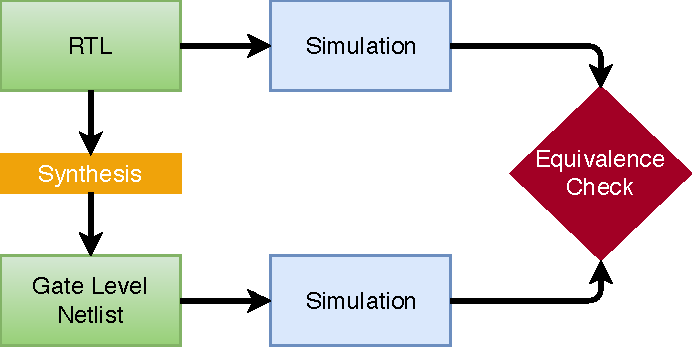
\includegraphics[width=0.7\textwidth]{Figures/Gate-level.pdf}
	\caption{Gate level design flow diagram.}
	\label{fig:gl}
\end{figure}

\subsection{Hardware-based Simulators}
\label{subsection:hardware}

As the name indicates, hardware-based simulators are a type of simulators that
rely on configurable hardware to do the digital circuit verification. When
compared with the software-based simulators, they have the advantage of being a
few orders of magnitude faster~\cite{tan:vhstas}. However they also have some
disadvantages: the hardware can be costly sometimes (depending on its
specifications) and it requires long compilation times, which makes them
needless for smaller designs. These simulators also require proprietary hardware
platforms to perform the desired simulations, with the hardware setup depending
on the platforms used, being different on each platform. As a result, these type
of simulators have a steep learning curve.

In this simulation type, the Verilog design is mapped onto a reconfigurable
piece of hardware with the same logical behavior as the netlist.  The simulation
is divided between the software simulator, which simulates all the Verilog code
that is not synthesizable, and the hardware accelerator, which simulates
everything that is synthesizable~\cite{khandelwal:gatelevel}. The design is then
run on the hardware, producing the simulation results. The results, like in a
Software-based simulator, must be checked in order to assess if the circuit is
working properly.

There are two variants of Hardware-based simulators: FPGA-based or
emulator-based. On one hand, the FPGA-based simulators, as the name indicates,
rely on FPGAs. A FPGA (Field Programmable Gate Array) is an integrated circuit
designed to be configured multiple times, according to the user needs. It
comprises an array of programmable logic blocks, memory elements, arithmetic
functions, etc.

The FPGA-based simulators follow the flow shown in Figure~\ref{fig:fpga}. The
original Verilog description of the code is transformed into an intermediate
representation, independent of the target platform. Here, the synthesizable
portions of the code are mapped into the FPGA, while the non synthesizable
portions (namely intendend for verification purposes) are run as software in the
host machine (software/hardware co-simulation). The simulator and the FPGA
interact with each other to produce the results.

\begin{figure}[!htb]
	\centering
	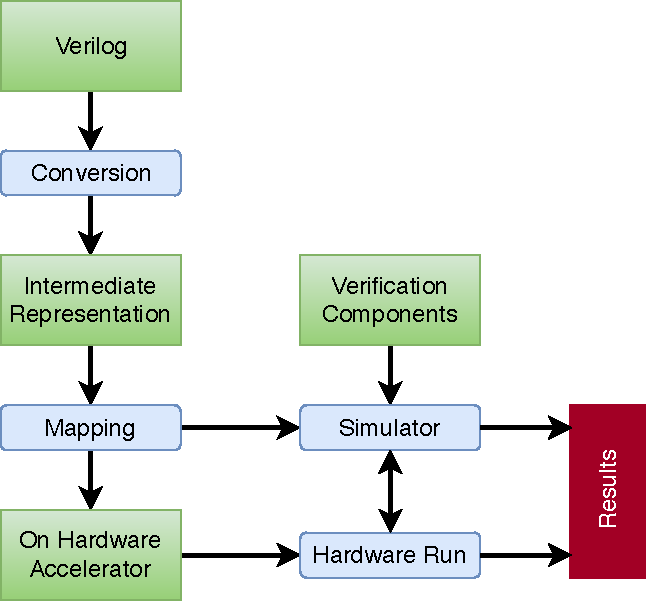
\includegraphics[width=0.7\textwidth]{Figures/FPGAsim.pdf}
	\caption{FPGA-based simulation flow~\cite{khandelwal:gatelevel}.}
	\label{fig:fpga}
\end{figure}

On the other hand, Emulator-based simulators rely on emulators to run their
simulations. An emulator is a specialized piece of hardware, that is , an
Application Specific Circuit (ASIC) that, when compared to a FPGA offers limited
reconfigurability, but with the advantage of a higher simulation speed. Even
though, the FPGA can run the actual circuit which in many cases superseeds
emulators in performance despite the lower clock frequency.

This type of simulation offers the possibility of testing software on the
developed design before having it implemented on chip, in a way that the
software application runs exactly as it would on the real chip in a real
circuit. It also offers the possibility for testing more complex programs, that
would take large amounts of time (sometimes even days) to run on other types of
simulators (like the software-based ones).

The simulation flow for this type of simulators has some similarities with the
FPGA-based simulators. In this case, as shown in Figure~\ref{fig:emulator}, the
Verilog code is converted into an intermediate representation, that will the be
mapped into the emulator. The code to be mapped must include only code that can
be implemented into the emulator. This means that the non synthesizable code
must be separated, being included in the software application. Both the software
and hardware platform interact with each other to produce the results.

\begin{figure}[!htb]
	\centering
	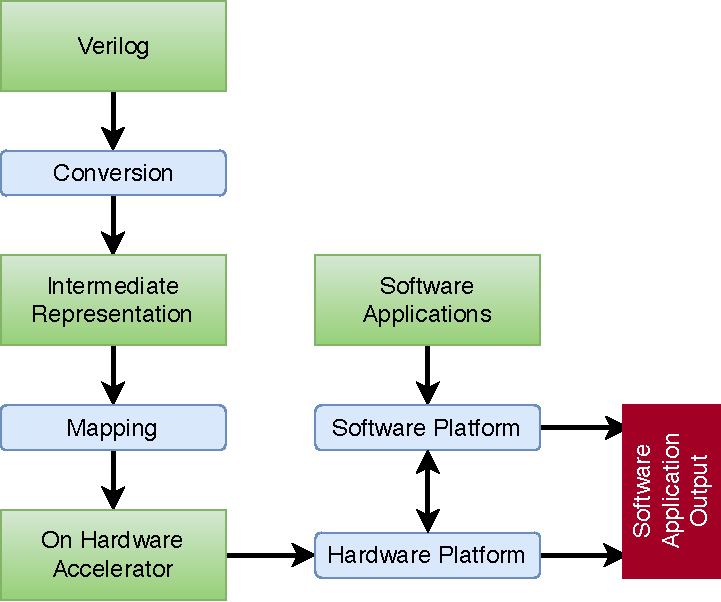
\includegraphics[width=0.7\textwidth]{Figures/Emulatorsim.pdf}
	\caption{Emulator-based simulation flow~\cite{khandelwal:gatelevel}.}
	\label{fig:emulator}
\end{figure}

\section{Cycle-Accurate Simulators}
\label{section:cycle}

Cycle-Accurate simulators are another important category of HDL
simulators. Instead of taking events sequentially, propagating them through the
circuit until it reaches a steady state, like the event-driven simulators, this
type of simulators evaluate each logic element of the circuit in a clock
cycle. They do this evaluation for each clock cycle, without taking into
consideration the propagation times and delays within the
cycle~\cite{khandelwal:gatelevel}.

As a result, these simulators are considerably faster than the event-driven
ones. However, they provide incomplete information about the circuit, since they
do not evaluate the delays and propagation times when evaluating each clock
cycle. So, if a circuit has timing problems, a cycle-accurate simulator will not
be able to notice them, making necessary the use of an even-driven simulator at
some stage to evaluate the existence of timing problems. All these
characteristics make the cycle-accurate simulators best suited for large circuit
simulation, like CPUs, when simulation speed is an important factor.

Most cycle-accurate simulators use a 2-state model (0 or 1) to calculate the
values of the signals through the circuit. A typical event-driven simulator uses
a more complex model, with more states (adding states like undefined, unknown or
high-impedance)~\cite{bennett:verilator}. This means that cycle-accurate
simulators have to make assumptions when the signals may have a value different
from 0 or 1 (for example, a signal that was uninitialized). While this speeds up
the simulation process, it also might be prone to produce wrong results.

From all the cycle-accurate simulators available, the most used one is probably
Verilator. Verilator is an open source simulator that compiles synthesizable
Verilog RTL, generating cycle accurate C++ and SystemC models. For each circuit, Verilator compiles a different model. These models are
then linked to a test bench, being executed in order to generate the
simulation. Verilator does not only translate Verilog code to C++ or
SystemC. Instead, it compiles the code into a much faster optimized and
thread-partitioned model, which is in turn wrapped inside a C++/SystemC
module~\cite{veripool:verilator}.

\section{Performance Comparison}
\label{section:performance}

When comparing event-driven and cycle-accurate simulators, not only their
working principles differ, but also their performance. Event-driven simulators
are typically slower than cycle-accurate simulators. This happens because the
algorithms used are more complex in event-driven simulators, having to implement
event scheduling and timing evaluation. The events are taken sequentially, being
propagated through the circuit until it reaches a steady state. New events
resultant from the output changes are added, meaning that the same element might
be evaluated multiple times during the same time step due to the feedback from
some signals. This whole process requires a considerable amount of time (and
computational power), being the main reason behind the lower speed of
event-driven simulators, when compared with cycle-accurate simulators.

The cycle-accurate simulators are typically the fastest type of simulators. This
happens because the simulation algorithm is simpler, evaluating each logic
element of the circuit in a clock cycle only once. They do this evaluation for
each clock cycle, without taking into consideration the propagation times and
delays within the cycle. There are also some simplifications that help improving
the simulation speed, like the use of a 2-state model (0 or 1) to calculate the
values of the signals through the circuit, instead of a model with multiple
states~\cite{bennett:verilator}.

In Figure~\ref{fig:performance} a graphic comparing the performance of the most
popular HDL simulators available in the market~\cite{verilator:benchmarks} is
shown. To run these benchmarks, a slightly modified model of the Motorolla M68K
processor was used. All the simulators shown were run in a general purpose
computer with an AMD Phenom 9500 2.2GHz processor, DDR2 667 Memory and running
the SuSE 11.1 operating system. The benchmark measures the number of cycles that
a simulator can run in a fixed amount of time, so a higher result means that
the simulator has a better performance.

From the analysis of the benchmark results, it can be concluded that Verilator
is considerably faster than the other tested simulators, both in 32 and 64 bits
versions. Cadence NCSim is almost 2 times slower than Verilator, while Synopsis
VCS is 3.5 times slower. Icarus Verilog is the slowest simulator tested, being
almost 80 times slower than Verilator. The benchmark results shown should only
work as reference, given their limitations: the versions of the simulators used
are already outdated, the same happening with the hardware and operating systems
used in the general purpose computers. Also, this benchmark only evaluates the
performance in one model (Motorolla M68K processor), instead of using multiple
models in order to provide more accurate results.

\begin{figure}[!htb]
	\centering
	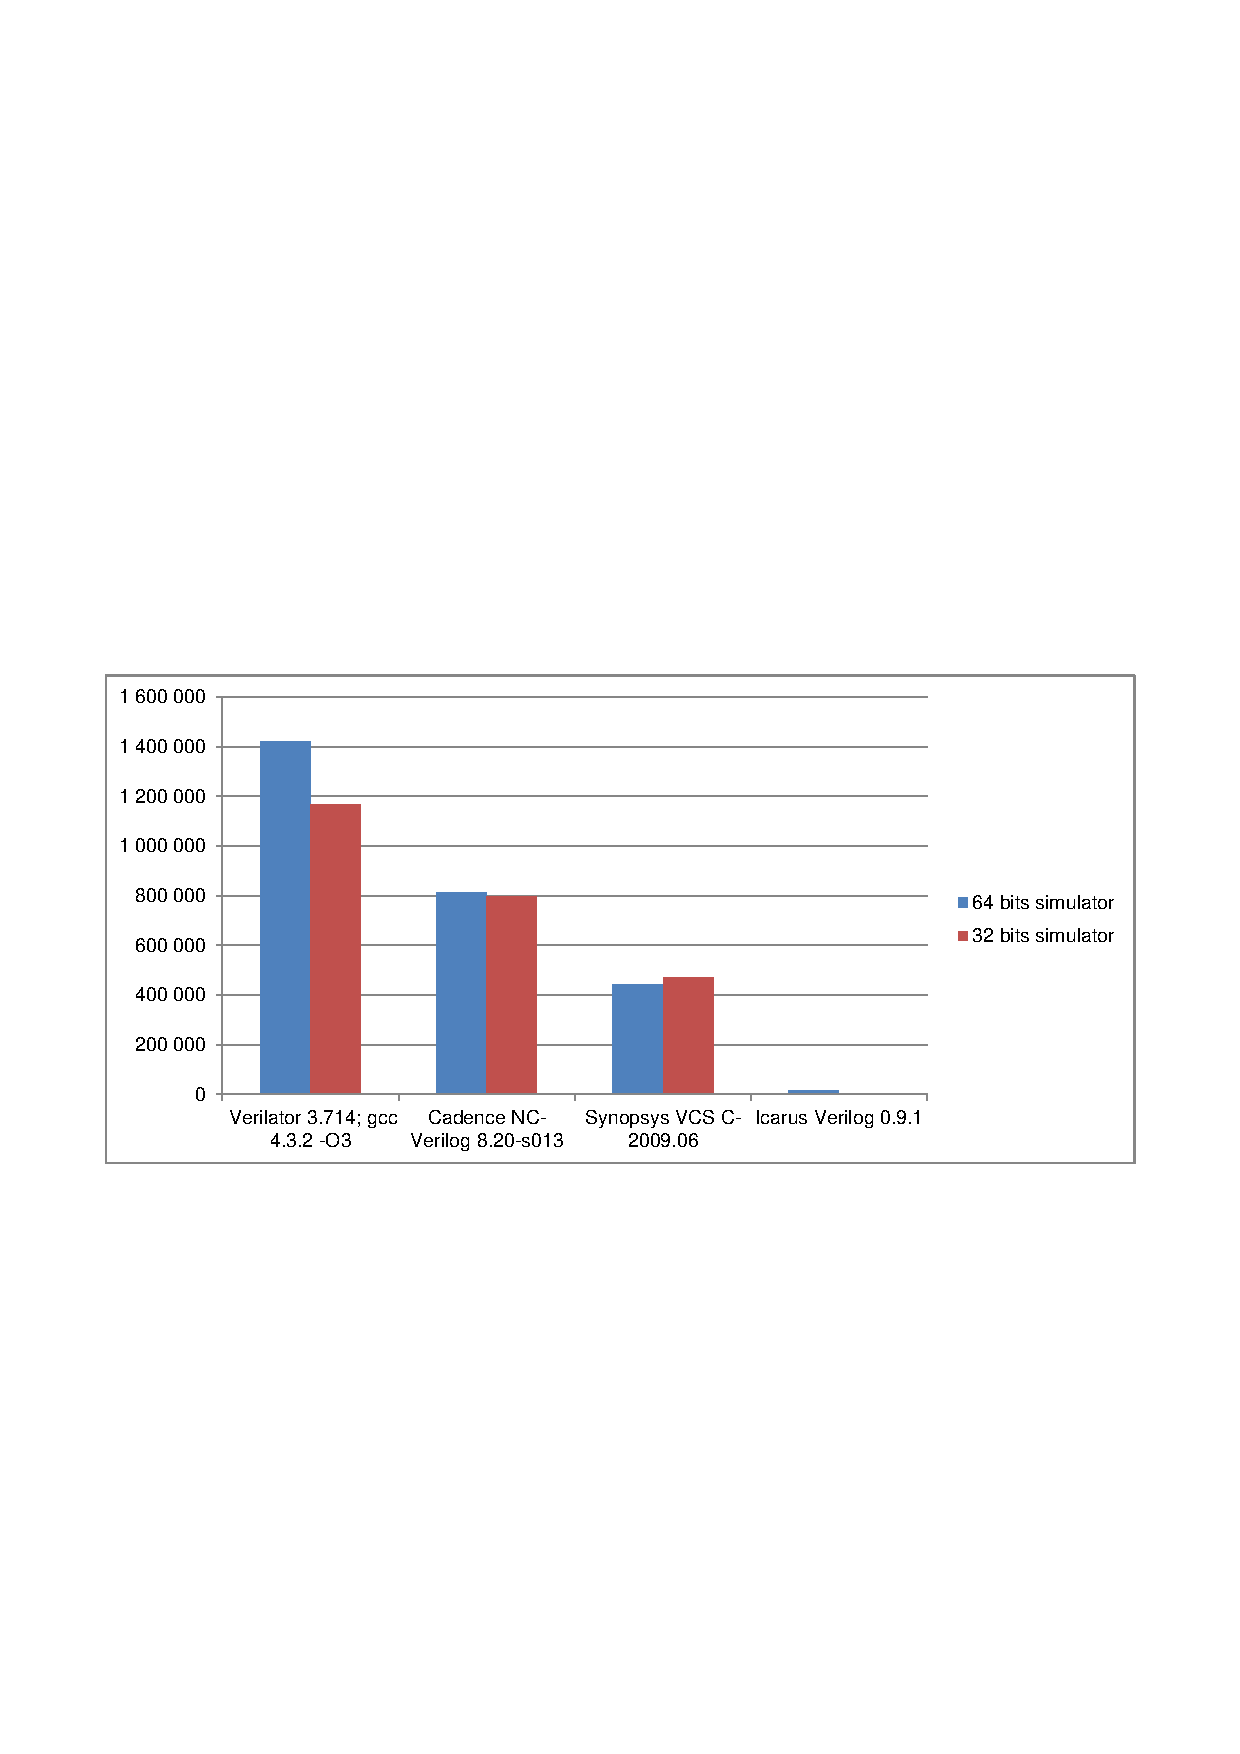
\includegraphics[trim=0 280 0 310 , clip, width=0.93\textwidth]{Figures/Performance.pdf}
	\caption{Benchmark results for different HDL simulators (higher means faster)~\cite{verilator:benchmarks}.}
	\label{fig:performance}
\end{figure}

The benchmark runs for the results shown in Figure~\ref{fig:performance} were
made in single-threaded mode. However, most commercial simulators (including the
ones analysed) support simulations in multi-threaded mode. This consists in
creating multiple threads for the different processes and distributing them
through multiple cores in a chip or even across multiple chips, that will be
executed in parallel. The threads are usually inter-dependent, so there should
be a synchronization process when transferring data between threads. This
process is time consuming, since different threads have different execution
times, requiring the faster threads to hold on until the slowest thread
finishes~\cite{tan:vhstas}.

Despite the concurrent nature of the Verilog statements, it isn't feasible to
parallelize the totality of the statements in a model, since the number of
statements is much greater than the amount of threads available, and also
because this would require a great amount of synchronization processes between
the different threads. Instead, the Verilog top-level code is divided in
multiple subsystems, with each one being simulated as a different thread.

The parallelization of HDL simulations is the solution found to achieve
considerable performance improvements in HDL simulators. This happens because
through the years the algorithms used in the simulators were optimized to such a
point where there were no further optimizations available, so the only viable
solution was to start using parallelization techniques.

%%  LocalWords:  parallelize
 % file "Thesis_Simulators.tex"
\cleardoublepage

%%%%%%%%%%%%%%%%%%%%%%%%%%%%%%%%%%%%%%%%%%%%%%%%%%%%%%%%%%%%%%%%%%%%%%%%
%                                                                      %
%     File: Thesis_Versat.tex                                      %
%     Tex Master: Thesis.tex                                           %
%                                                                      %
%     Author: Andre C. Marta                                           %
%     Last modified :  2 Jul 2015                                      %
%                                                                      %
%%%%%%%%%%%%%%%%%%%%%%%%%%%%%%%%%%%%%%%%%%%%%%%%%%%%%%%%%%%%%%%%%%%%%%%%

%JTS: replace ' ' with '~' between word and \ref or \cite in the whole document
%not only in this file

\chapter{CGRA Simulation}
\label{chapter:CGRA}

As referred before in this work, CGRA architectures have some big differences
when compared with dedicated circuits. This poses difficulties in some areas,
with one of these areas being the simulation of the developed
architectures. Unlike a dedicated circuit, in a CGRA the reconfigurable
interconnects between the functional units allow to build zillions of different
datapaths at run-time. This is an overhead compared to simulating the various
datapaths separately without simulating the reconfigurable infrastructure.

For FPGAs this problem is even worse as the reconfigurable infrastructure is
fine grain and there are small Look Up Tables (LUTs) instead of high-level FUs
like in CGRAs, and even more programmable interconnects. For this reason the
FPGA fabric is never simulated, only the circuits that are mapped onto it are.

As a result, simulating CGRAs with event-driven simulators will result in
lengthy simulation times. Consequently, finding a valid alternative to simulate
CGRAs (in this particular case, the Versat architecture) could save an important
amount of time and money during the development of applications for this type of
architectures.

Using cycle-accurate simulators could be a good alternative to speed up CGRA
simulations. As seen in the previous chapter, the use of a cycle-accurate
simulator like Verilator could cut considerably the simulation time, reducing
it, at least, by a factor of 2 (see Fig~\ref{fig:performance}). It also has the
advantage of having no additional cost, since Verilator is open source. However,
the CGRA (or any other circuit) should not be tested exclusively with a
cycle-accurate simulator, since their results don't have in account the
propagation delays inside the CGRA, and also make some simplifications regarding
the signals state. This is specially true if the CGRA is in constant development
as is the case for Versat.

Another alternative is doing simulations at a high-level, instead of doing them
at the RTL level. High-level simulation techniques have been applied in
different types of circuits, like processors, with good results. However, for
CGRA there is an additional difficulty compared to regular processors for this
type of simulations because of the reconfiguration process. Two examples of
approaches to high-level simulation are presented next: one that proposes a
cycle-accurate simulator~\cite{chen:CGRA}, and another one that proposes a
framework for high-level simulation of CGRAs~\cite{pasha:CGRA}.


\section{High-level cycle-accurate simulator}
\label{section:hlcycle}

The high-level cycle-accurate approach proposed in~\cite{chen:CGRA} introduces
the concept of a timing-constrained datapath. In CGRAs there is not a well
defined pipeline structure due to the reconfigurable interconnects. The pipeline
is formed on the fly with registers or memories being used to save the
intermediate results between the different datapaths.

With this in mind, a register-centric synthesis technique is used using a
timing-constrained datapath rooted at a chosen register. For the example in
Figure~\ref{fig:datapaths}, the datapath is rooted at the register R0, with the
different paths being tracked down within the timing constraint given. These
datapaths can finish either on a circuit input or on an intermediate register.

\begin{figure}[!htb]
	\centering
	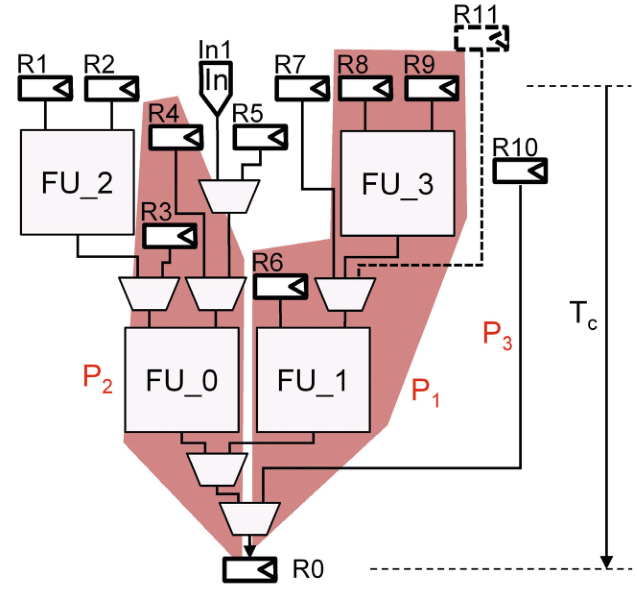
\includegraphics[width=0.6\textwidth]{Figures/Datapaths.png}
	\caption{Timing-constrained datapath example~\cite{chen:CGRA}.}
	\label{fig:datapaths}
\end{figure}

The timing-constrained datapaths will be extracted and used by the compiler,
being converted into a pattern graph of FUs. In this way, the simulation becomes
a signal flow graph simulation, being performed via a routine that updates the
value of all registers and output ports on each clock cycle. For the
register/port udpate routine the obtained graph will be traversed, starting on
the root register, and evaluating all the possible paths. This means that the
simulator only does the necessary operations for the existent configuration
bits, and also that the worst case for the simulation execution time will be
proportional to the number of configuration bits available on the longest path
of the flow graph.

The main simulation routine uses three main components: Input Read,
Register/Port Update (described previously) and State Update. The Input Read is
responsible for reading all the inputs on each clock cycle, and the
Register/Port Update for updating all the values of registers that need to be
updated.

%JTS: what about State Update?

To evaluate the performance of this simulator, multiple simulations were made,
using two different CGRAs: CGRA-1 (modelled similarly to ADRES architecture~\cite{mei:reconfigurable}) and CGRA-2 (similar to~\cite{chen:flexdet}), and
running six different application kernels (3 on each CGRA). Those kernels were
run with different timing constraints, being noted that, while in CGRA-1 the
simulation time increased linearly with the timing constraint, in CGRA-2 the
simulation time did not increase so much. This happened because the CGRA-2 had a
well defined pipeline architecture, along with less complex interconnections.

%JTS: did not get this. Are you sure you understand this?

The simulations speed was compared with some commercially available simulators
(Synopsys VCS-MX 2011.03 and Verilator 3.853), using a system with an AMD Phenom
II X4 955 CPU and 8 GB of memory. To run the simulations the timing constraint
was set to 3 FUs, since the performance of the kernels is the same as without
timing constraint. Both the generated high-level simulator and Verilator were
compiled with GCC 4.4.7. The obtained results are shown in Figure~\ref{fig:hlperformance}, normalized with the simulation time for the high-level
simulator.

\begin{figure}[!htb]
	\centering
	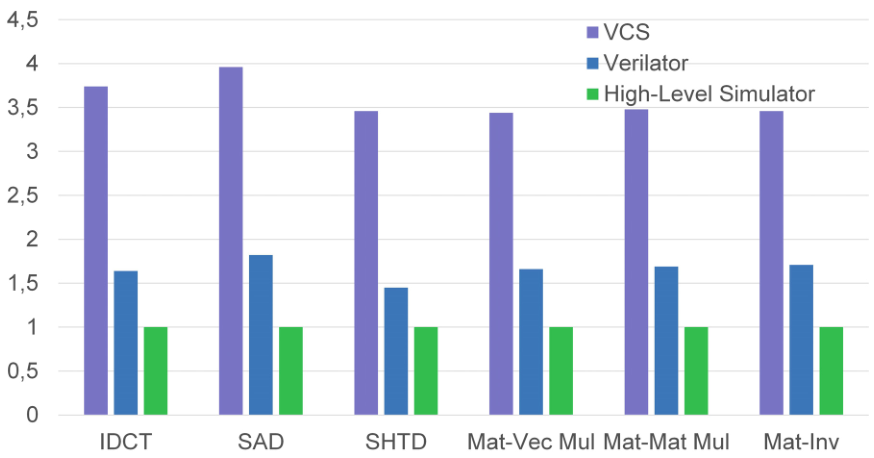
\includegraphics[width=0.8\textwidth]{Figures/hlperformance.png}
	\caption{Performance comparison between the high-level and other commercially available simulators~\cite{chen:CGRA}.}
	\label{fig:hlperformance}
\end{figure}

From the results in Figure~\ref{fig:hlperformance} it can be seen that the
high-level simulator is almost 4 times faster than Synopsys VCS and around 1.5
times faster than Verilator. This was already expected given that, while the
high-level simulator only considers the values in the registers after each
execution cycle, the other simulators also evaluate the intermediate signals.

\section{CGRA high-level simulation framework}
\label{section:framework}

The framework presented in~\cite{pasha:CGRA} provides a high-level simulation
and optimization solution for a given mesh-based CGRA. It accepts applications
written in C, generating the corresponding VHDL description for the target CGRA,
and it can be divided into two main parts: C to netlist transformation and
netlist to CGRA mapping.

The C to netlist transformation relies on GeCoS~\cite{l'hours:FPGA}, an
open-source compiler mainly used for ASIPs (Application Specific Instruction Set
Processors) to compile the C code, generating a data flow graph that represents
the original C code. This was made using GeCoS direct acyclic graphs generation
capabilities. To transform the generated graphs into netlists for the target
CGRA, a parser was created. In the resulting netlist, each ALU corresponds to a
node in the original graph.

For the netlist to CGRA mapping, the previously generated netlists are placed
into the target CGRA, using a simulated annealing algorithm. The placement and
routing algorithms for netlist to CGRA mapping used are independent of the CGRA
architecture, so they can be used for exploring different architectures. In the
end an estimation of the area used is calculated.

The performance of the developed framework was only compared with FPGAs, using
an open-source high-level simulation tool targeted at FPGA generation.
%JTS: what tool? why does the fpga need to be generated ?
However, instead of comparing the CGRA simulation performance with the FPGA
simulation
%JTS: or execution ?
performance, it would be more useful (in the scope of this report) to compare
how this new framework performs simulating a CGRA when compared with other
commercial HDL simulators, using the same architecture.
 % file "CGRA_Simulation.tex"
\cleardoublepage

%\input{Thesis_new_file} % add new .tex files for new chapters
% \cleardoublepage

%\input{Thesis_new_file} % add new .tex files for new chapters
% \cleardoublepage

%\input{Thesis_new_file} % add new .tex files for new chapters
% \cleardoublepage

%%%%%%%%%%%%%%%%%%%%%%%%%%%%%%%%%%%%%%%%%%%%%%%%%%%%%%%%%%%%%%%%%%%%%%%%
%                                                                      %
%     File: Thesis_Conclusions.tex                                     %
%     Tex Master: Thesis.tex                                           %
%                                                                      %
%     Author: Carlos A. Rodrigues                                      %
%     Last modified : 21 Jan 2011                                      %
%                                                                      %
%%%%%%%%%%%%%%%%%%%%%%%%%%%%%%%%%%%%%%%%%%%%%%%%%%%%%%%%%%%%%%%%%%%%%%%%

\chapter{Conclusão}
\label{chapter:conclusao}

Insert your chapter material here...


% ----------------------------------------------------------------------
\section{Achievements}
\label{section:achievements}

The major achievements of the present work...


% ----------------------------------------------------------------------
\section{Trabalho Futuro}
\label{section:futuro}

dese


\cleardoublepage

 % file "Thesis_Conclusions.tex"
\cleardoublepage

% ----------------------------------------------------------------------
%  Bibliography
% ----------------------------------------------------------------------

% Add entry in the table of contents as chapter
\phantomsection
\addcontentsline{toc}{chapter}{\bibname}

% Include all references in .bib file, even non-cited ones...
%\nocite{*} % this should be used carefully because it is not correct!

% Produces the bibliography section when processed by BibTeX
%
% Bibliography style
% > entries ordered alphabetically
%\bibliographystyle{plain}
% > unsorted with entries appearing in the order in which the citations appear.
%\bibliographystyle{unsrt}
% > entries ordered alphabetically, with first names and names of journals and months abbreviated
%\bibliographystyle{abbrv}
% > entries ordered alphabetically, with reference markers based on authors' initials and publication year
%\bibliographystyle{alpha}
%
% Replacement bibliography styles provided by 'natbib' package
% (plainnat.bst, abbrvnat.bst, unsrtnat.bst )
% > entries ordered alphabetically
%\bibliographystyle{plainnat}
% > unsorted with entries appearing in the order in which the citations appear.
%\bibliographystyle{unsrtnat}
% > entries ordered alphabetically, with first names and names of journals and months abbreviated
%\bibliographystyle{abbrvnat} % <<<<< SELECT IF USING REFERENCES BY AUTHOR/YEAR
% > entries ordered alphabetically, with reference markers based on authors' initials and publication year
%\bibliographystyle{alpha}
%
% Custom bibliography style adapted from 'natbib' package
%   (based on http://tex.stackexchange.com/questions/5053/is-it-possible-to-get-unsrt-abbrv-bibliography)
%   (unsrtnat.bst + abbrvnat.bst -> abbrvunsrtnat.bst)
%   (original files copied from:
%   http://tug.ctan.org/macros/latex/contrib/natbib/abbrvnat.bst
%   http://tug.ctan.org/macros/latex/contrib/natbib/unsrtnat.bst
% > unsorted with entries appearing in the order in which the citations appear, with first names and names of journals and months abbreviated.
\bibliographystyle{abbrvunsrtnat} % <<<<< SELECT IF USING REFERENCES BY NUMBER (CITATION ORDER)

% External bibliography database file in the BibTeX format
\bibliography{Thesis_bib_DB} % file "Thesis_bib_DB.bib"

\cleardoublepage

% ----------------------------------------------------------------------
%  Appendix (optional)
%
%  CAUTION: 1) the main document (up to the conclusions) shall not exceed 80 pages
%           2) the document shall not exceed a total of 100 pages (per IST regulations)
% ----------------------------------------------------------------------
\appendix

% add page number prefix according to apendix chapter (optional)
%\renewcommand{\thepage}{\thechapter.\arabic{page}}

% re-set arabic numbering (A.1,A.2,...) (optional, use only if chapter prefix is added)
%\setcounter{page}{1}

%%%%%%%%%%%%%%%%%%%%%%%%%%%%%%%%%%%%%%%%%%%%%%%%%%%%%%%%%%%%%%%%%%%%%%%%%
%                                                                      %
%     File: Thesis_Appendix_A.tex                                      %
%     Tex Master: Thesis.tex                                           %
%                                                                      %
%     Author: Andre C. Marta                                           %
%     Last modified :  2 Jul 2015                                      %
%                                                                      %
%%%%%%%%%%%%%%%%%%%%%%%%%%%%%%%%%%%%%%%%%%%%%%%%%%%%%%%%%%%%%%%%%%%%%%%%

\chapter{Vector calculus}
\label{chapter:appendixVectors}

In case an appendix if deemed necessary, the document cannot exceed a total of 100 pages...

Some definitions and vector identities are listed in the section below.

% ----------------------------------------------------------------------
\section{Vector identities}
\label{section:vectorIdentities}

\begin{equation}
	\nabla \times \left( \nabla \phi \right) = 0
	\label{eq:cross_nnp}
\end{equation}

\begin{equation}
	\nabla \cdot \left( \nabla \times {\bf u} \right) = 0
	\label{eq:dotCross_nnu}
\end{equation}

 % file "Thesis_Appendix_A.tex"
%\cleardoublepage

% re-set arabic numbering (B.1,B.2,...) (optional, use only if chapter prefix is added)
%\setcounter{page}{1}

%%%%%%%%%%%%%%%%%%%%%%%%%%%%%%%%%%%%%%%%%%%%%%%%%%%%%%%%%%%%%%%%%%%%%%%%%
%                                                                      %
%     File: Thesis_Appendix_B.tex                                      %
%     Tex Master: Thesis.tex                                           %
%                                                                      %
%     Author: Andre C. Marta                                           %
%     Last modified :  2 Jul 2015                                      %
%                                                                      %
%%%%%%%%%%%%%%%%%%%%%%%%%%%%%%%%%%%%%%%%%%%%%%%%%%%%%%%%%%%%%%%%%%%%%%%%

\chapter{Technical Datasheets}
\label{chapter:appendixDatasheets}

It is possible to add PDF files to the document, such as technical sheets of some equipment used in the work.

% ----------------------------------------------------------------------
\section{Some Datasheet}
\label{section:datasheet}

% See more options to include PDF files in
% http://mirror.unl.edu/ctan/macros/latex/contrib/pdfpages/pdfpages.pdf
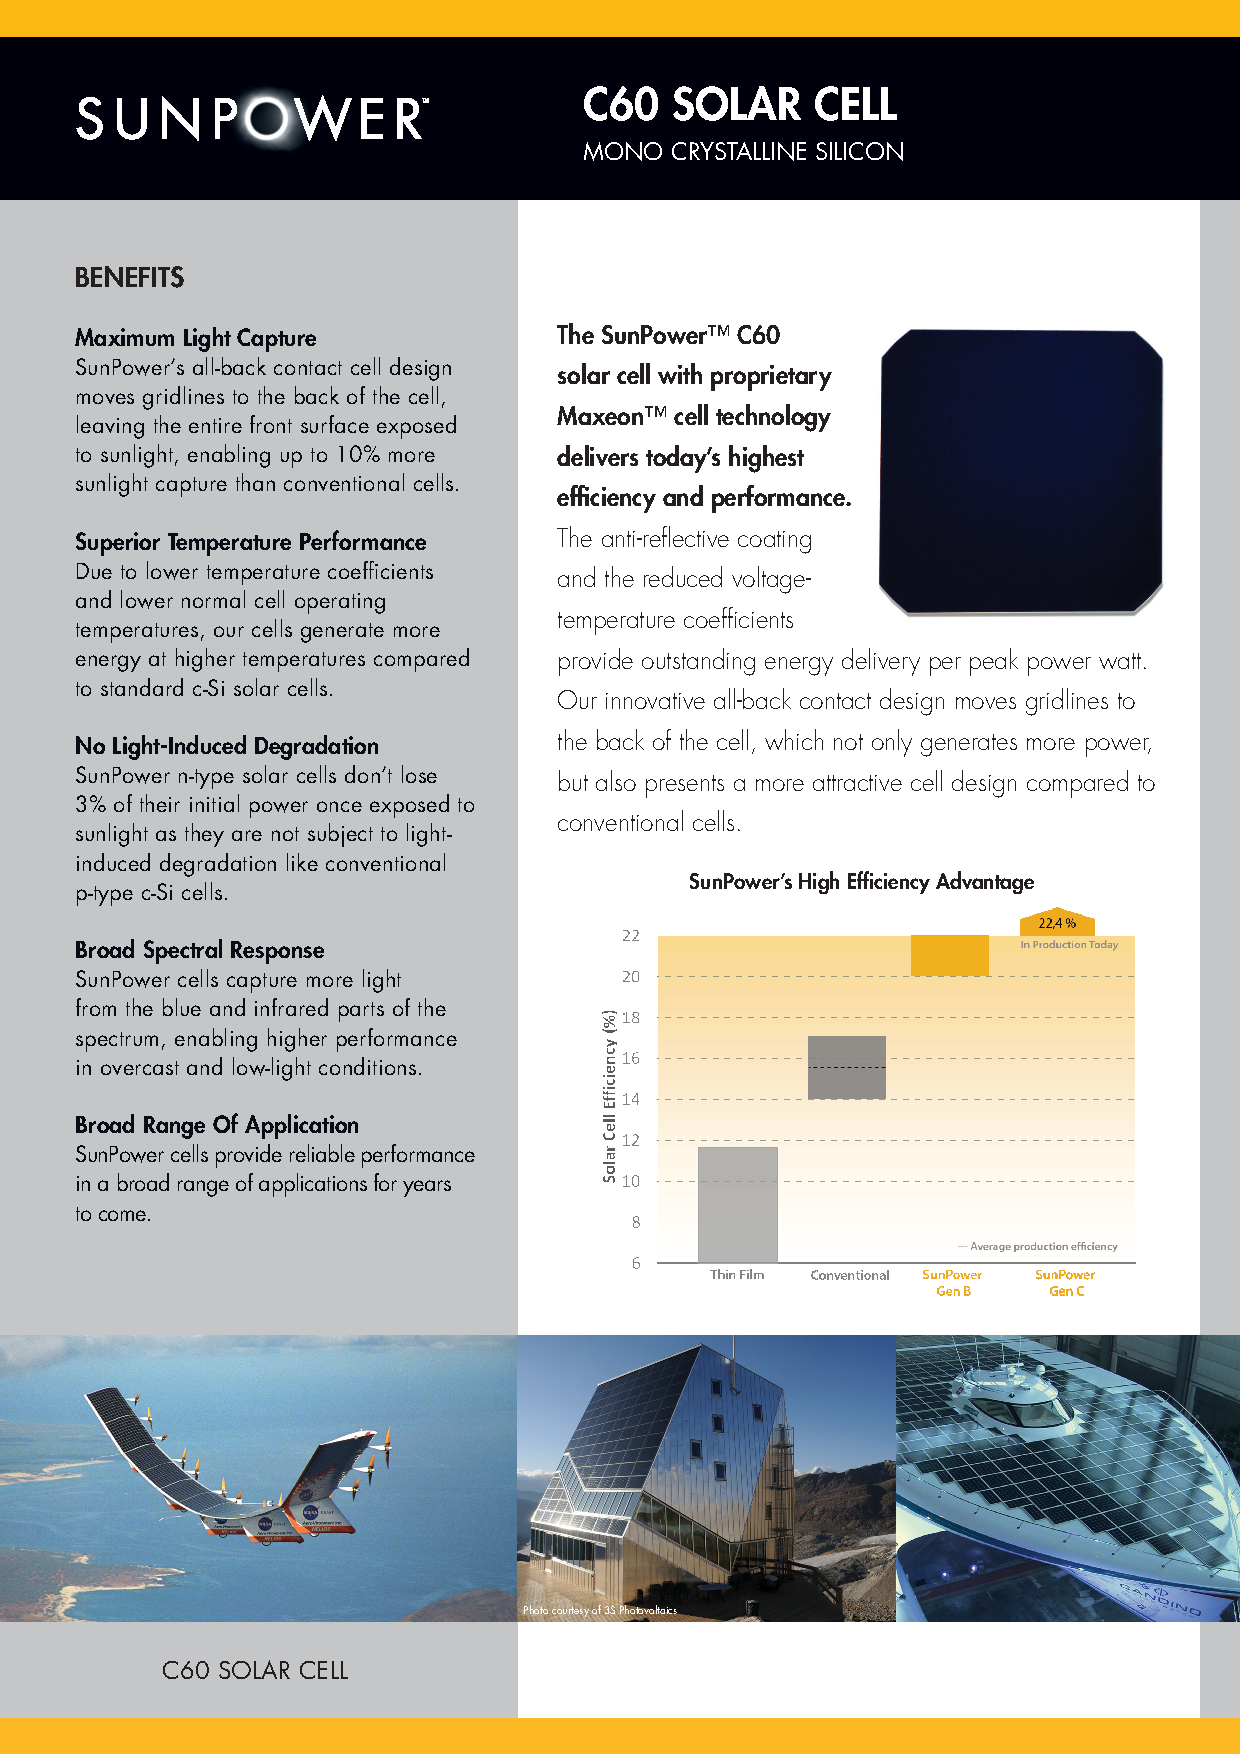
\includepdf[pages={1-2},nup=1x2,landscape=true]{Figures/SolarCell_Sunpower_C60.pdf}

 % file "Thesis_Appendix_B.tex"
%\cleardoublepage

% ----------------------------------------------------------------------
\end{document}
% ----------------------------------------------------------------------

